%%%%%%%%%%%%%%%%%%%%%%%%%%%%%%%%%%%%%%%%%%%%%%%%%%%%%%%%%%%%%%%%%%%%%%%%%%%%%%
%	Plantilla para Memorias y Tesis, UTFSM, Chile
%	=============================================
%
% Autor:
%       Jaime C. Rubin-de-Celis <jaime@rubin-de-celis.com>
%
% Fecha:	
%       $Date: 2017-10-28 11:25:21 -0300 (Sat, 28 Oct 2017) $
%
% Versión:
%       1.1
%
% Licencia:
%       Copyright (c) 2012-2017, Jaime C. Rubin-de-Celis
%       The MIT License
%
% Nota:
%       Las imágenes son propiedad intelectual de la UTFSM.
%
% Uso:
%       Ver archivo adjunto README.md.
%       Si todo lo demás falla, recuerde "RTFM".
%
%%%%%%%%%%%%%%%%%%%%%%%%%%%%%%%%%%%%%%%%%%%%%%%%%%%%%%%%%%%%%%%%%%%%%%%%%%%%%%

\documentclass[
	12pt,			% Tamaño de fuente (11pt)
	letterpaper,	% Tamaño del papel (carta)
	oneside,		% Doble Cara
]{thesis_utfsm}

\usepackage{thesis_utfsm}   % Archivo de estilos 

%!TEX root = memoria.tex

%---------------------------------------------------------------------------
%%% CONFIGURACIÓN
%---------------------------------------------------------------------------
%
%%% CODIFICACIÓN DE CARACTERES
% Este documento está escrito usando caracteres Unicode (UTF8)
% Por lo que la siguiente línea es necesaria para reconocer los acentos
% y otros caracteres en español.
% Si ve caracteres extraños en el PDF (en Windows o MAC) pruebe 
% con alguna de estas líneas:
\usepackage[utf8x]{inputenc}    % *nix / Linux / MacOSX
%\usepackage[latin1]{inputenc}  % Windows (MacOSX)


\newcommand{\TheTitle}           {PLAN DE CALIDAD PARA GERPRIN}
\newcommand{\TheAuthor}          {GABRIEL ARÍSTIDES CAMILO SAN MARTÍN}
\newcommand{\TheGrade}           {INGENIERO DE EJECUCIÓN EN INFORMÁTICA}
\newcommand{\TheCity}            {SANTIAGO}
\newcommand{\TheDate}            {OCTUBRE 2018}
\newcommand{\TheAdvisor}         {MARCELLO VISCONTI ZAMORA}
\newcommand{\TheCoAdvisor}       {LIOUBOV DOMBROVSKAIA}

% Marca de agua, puede ser deshabilitada para impresión rápida
\insertWatermark{figures/logousm_watermark.jpg}
%---------------------------------------------------------------------------


%---------------------------------------------------------------------------
%%% No editar (¡Ver licencia!) (MIT License, 2016)
%---------------------------------------------------------------------------
\hypersetup{  
    pdfinfo={  
        Subject={Memoria Departamento de Industria, UTFSM},
        Keywords={Memoria} {Departamento de Industrias} {UTFSM},
        Producer={JCR LaTeX Templates, http://www.rubin-de-celis.com/},
        Licence={http://www.rubin-de-celis.com/LICENSE},
        pdfpagemode=FullScreen,
        pdfmenubar=false,
        pdftoolbar=false
    }  
}
\hypersetup{  
    pdfinfo={  
        Title={\TheTitle},
        Author={\TheAuthor}
    }  
}
%---------------------------------------------------------------------------              % Configuración (Título, autor, etc.)
                            % Usted debe modificar este documento
                            % para actualizar la portada.

\makeatother                % Important! (Do not delete or move!)


% Generadores de texto aleatorio (se pueden eliminar)
\usepackage{blindtext}      % automated text generation
\usepackage{lipsum}         % automated text generation


%---------------------------------------------------------------------------
%%%%%%%%%%%%%%%%%%%%%%%%%%%%%%%%%%%%%%%%%%%%%%%%%%%%%%%%%%%%
%	Documento
%%%%%%%%%%%%%%%%%%%%%%%%%%%%%%%%%%%%%%%%%%%%%%%%%%%%%%%%%%%%
\begin{document}

\pagestyle{plain}           % Headers & Footers (Roman numbers)

%---------------------------------------------------------------------------
%%%%%%%%%%%%%%%%%%%%%%%%%%%%%%%%%%%%
%	Portada
%%%%%%%%%%%%%%%%%%%%%%%%%%%%%%%%%%%%
\insertFile{portada}        % Insertar archivo 'sections/portada.tex'.

%---------------------------------------------------------------------------
%%%%%%%%%%%%%%%%%%%%%%%%%%%%%%%%%%%%
%	Preámbulo (Front Matter)
%%%%%%%%%%%%%%%%%%%%%%%%%%%%%%%%%%%%
\frontmatter                % Important! (Do not delete or move!)


\insertFile[plain]{resumen}     % Insertar 'sections/resumen.tex'.

%%% TABLA DE CONTENIDOS / FIGURAS / CUADROS
\begin{spacing}{1}      % Single space for TOC, LOF and LOT
    \tableofcontents\listoftables\listoffigures
\end{spacing}



%---------------------------------------------------------------------------
%%%%%%%%%%%%%%%%%%%%%%%%%%%%%%%%%%%%
%	Cuerpo Principal (Main Matter)
%%%%%%%%%%%%%%%%%%%%%%%%%%%%%%%%%%%%
\mainmatter             % Important! (Do not delete or move!)

\pagestyle{fancy}       % Headers & Footers (Arabic numbers)

% Incluir Capítulos
%!TEX root = ../memoria.tex

\chapter{Introducción}
Considerando el prototipo de \textit{Gerprin} desarrollado para la XXIII Feria de Software de la Universidad Técnica Federico Santa María en año 2015, se busca crear un plan de calidad para el desarrollo de una nueva versión de este con propósitos comerciales, y así lograr un producto con estándares de calidad adecuados al mercado y asegurar un correcto funcionamiento de la nueva versión del sistema.

Es menester comenzar contextualizando el problema que se busca solucionar mediante la invención de \textit{Gerprin}, antes de proceder con una descripción preliminar del plan de calidad que se busca realizar. 

\section{Resumen del proyecto}

El Informe Anual entregado por Carabineros de Chile (Chile, 2018) contabilizó un total de 16.678 robos de vehículos motorizados entre los meses de enero y agosto. Esto significa que se sustrajo un vehículo, en nuestro país, cada 21 minutos.

En respuesta a lo anterior, nace \textit{Gerprin}, que busca eliminar la inseguridad en los conductores y permitir que puedan aparcar en cualquier lugar sin miedo a ser víctimas del robo de su vehículo. Para lograr esto, fue propuesto un sistema de seguridad vehicular integral que cuenta con tres aspectos. En primer lugar, un sistema a bordo de corta corriente controlado con un lector biométrico para que ningún extraño pueda operar el vehículo. En segundo lugar, un sistema centralizado de monitoreo de la posición \textit{GPS} del vehículo que genera alertas al cliente cuando se detectan movimientos no autorizados. Y finalmente, se desarrolló una aplicación móvil que le permitirá a nuestros clientes monitorear la posición de su vehículo y controlar el sistema a bordo, permitiendo agregar, modificar o eliminar usuarios de una forma fácil y rápida.

Con \textit{Gerprin} se buscó solucionar una de las necesidades más básicas del ser humano: la seguridad. No sólo se creó un gadget antirrobo, sino que gestó un completo sistema de protección para el automóvil, el cual entregará confianza y tranquilidad a los usuarios cuando deban estacionar sus vehículos en lugares que no conocen o incluso en su propio hogar. Con \textit{Gerprin} de monitoreo podrán saber en todo momento cual es la posición de su automóvil, mientras que, con el sistema biométrico, tendrán la certeza de que nadie podrá utilizar el vehículo sin su autorización.

 En último lugar, para comprender la envergadura del sistema es necesario señalar las diferencias con los productos del mercado. Señalar, además, que ya existen sistemas de corta corriente, incluso los hay operados con biometría; Los sistemas de monitoreo \textit{GPS} ya se han masificado y especialmente en el área de transporte comercial. \textit{Gerprin} representa un sistema de seguridad integral que combina todos los aspectos anteriores: la seguridad a bordo (corta corriente con biometría), monitoreo satelital centralizado (\textit{GPS}) y el control de estos mediante una aplicación móvil fácil de utilizar.

\section{Propósito}

Como fue mencionado al comienzo del presente documento, este trabajo busca realizar una segunda iteración en el desarrollo de \textit{Gerprin}, con el fin de generar una versión comercializable del sistema utilizando como punto de partida la primera iteración diseñada y desarrollada para la XXIII feria de software de la Universidad Técnica Federico Santa María.

En el presente plan de calidad se tiene como propósito establecer los procesos y acciones para el aseguramiento de calidad, definiendo la estructura para el desarrollo del sistema, las gestiones necesarias para dicho desarrollo, las herramientas y técnicas a emplear y las pruebas necesarias para asegurar la calidad esperada.

\section{Alcance}

El plan de calidad abordará las distintas etapas de ingeniería de software, desde un punto de vista práctico, enfocado a los productos y desarrollo de los pasos de análisis de requerimientos, diseño, desarrollo pruebas y documentación.

Dada la existencia previa de un software funcional desarrollado el año 2015 que cumple con los requisitos funcionales especificados para dicha aplicación, el presente plan de calidad se enfocará en los requisitos no funcionales.
%!TEX root = ../memoria.tex

\chapter{Requisitos no funcionales}

Se hace menester comenzar el plan de calidad definiendo los “atributos de calidad”, los indicadores de medición y los valores de validación de estos. Lo anterior, con el fin de definir los márgenes generales en el desarrollo de la aplicación y el nivel de integración del sistema con los atributos antes mencionados.

\section{Definición de atributos de calidad}

A continuación, se procederá con la presentación y definición de los requisitos no funcionales que definirán el lineamiento del desarrollo de la aplicación.

\begin{description}

\item[Fiabilidad:]\hfill

Se debe garantizar la respuesta de la aplicación ante una acción del usuario y además que la información entregada sea correcta.

\item[Usabilidad:]\hfill

Facilidad en el uso de la aplicación, reflejándose en la rapidez para aprender el funcionamiento del sistema y recordar este aprendizaje.

\item[Adapabilidad:]\hfill

Capacidad de la aplicación de funcionar en distintos entornos informáticos.

\item[Temporización:]\hfill 

Debe emplear el menor tiempo posible en entregar una respuesta visible al usuario ante una acción de este.

\item[Soportar alta carga:]\hfill 

El Sistema debe ser capaz de funcionar incluso en momentos de alto tráfico. 

\item[Disponibilidad:]\hfill 

El sistema debe encontrarse disponible para su acceso o consulta el mayor tiempo posible.

\item[Seguridad:]\hfill 

Protección de la infraestructura e información contenida en el sistema.

\item[Escalabilidad:]\hfill 

Capacidad del sistema de aumentar la carga de trabajo o sus funciones sin ver afectado el funcionamiento del resto de funcionalidades y tampoco disminuir su calidad.

\item[Mantenibilidad:]\hfill

 Esfuerzo y tiempo dedicado al soporte del sistema.

\end{description}

\section{Objetivos Cuantificables}

En la presente sección se establecerán los indicadores de cada uno de los atributos de calidad definidos en el apartado anterior. Además, se establecen los valores mínimos y máximos de los indicadores de los atributos de calidad, con el propósito de establecer de forma objetiva el cumplimiento requisitos no funcionales deseados en el sistema.

\subsection{Fiabilidad}

Es necesario que la información entregada por cualquiera de los distintos módulos que forman \emph{Gerprin} sea legible por los módulos restantes y de este modo no tener perdidas en la comunicación entre distintas plataformas. Las solicitudes y respuesta deben ser verídicas y corresponder a acciones reales desencadenadas por los actores de la aplicación.

Para lo anterior es necesario que el sistema de comunicación que se desarrollará no presente perdidas de información, sin embargo, se deben fijar estándares distintos para cada módulo respecto a la fiabilidad de los datos, debido a que la información que maneja la aplicación tiene distintos grados de importancia, incluso permitiendo perdida parcial de esta en determinadas condiciones.

Comenzando con el sistema a bordo, es necesaria la comunicación fiable con la \emph{API} de \emph{Gerprin} al momento de realizar activación o desactivación del cortacorriente mediante la aplicación móvil, pero no lo es para establecer una conexión fiable cada vez que el módulo contenedor del \emph{GPS} envía la posición. Por este motivo el envío de la ubicación se realiza mediante protocolo \emph{UDP}\footnote{https://www.ietf.org/rfc/rfc768.txt} , a diferencia del resto de las funciones del sistema a bordo que deben emplear \emph{TCP}\footnote{https://tools.ietf.org/html/rfc793}.

Por otro lado, la aplicación móvil y la \emph{API} desarrollada, deben contar con una conexión fiable de comunicación, esto debido a la información critica que es manejada por estos módulos.

\subsubsection{Objetivos cuantificables}

\begin{itemize}
	\item
	Funcionalidades de la aplicación móvil sin errores.
	\item
	Servicios entregados por la \emph{API} sin errores.
	\item
	Envió de posición de forma precisa e intervalos regulares sin errores.
	\item
	Funcionalidad de activación y desactivación de relé de forma remota sin errores.
\end{itemize}

\subsubsection{Criterios de medición.}

\begin{table}[H]
    \caption[Validación para los indicadores de fiabilidad.] {Validación para los indicadores de fiabilidad.}
    \label{tbl:Criterios de Validación fiabilidad}
    \begin{tabular}{|p{.6\textwidth}|p{.34\textwidth}|}
        \hline
        \textbf{Criterio} &  \textbf{Medición}\\
    	\hline
    	\hline
    	Funcionalidades de la aplicación móvil sin errores. & 95\% de efectividad sin errores. \\ \hline
		Servicios entregados por la \emph{API} sin errores. & 95\% de respuestas sin errores. \\ \hline
		Envió de posición de forma precisa e intervalos regulares sin errores. & 75\% de posiciones almacenadas con un error de ±20 metros. \\ \hline
		Funcionalidad de activación y desactivación de relé de forma remota sin errores. & 95\% de efectividad. \\
        \hline
    \end{tabular}
\end{table}

Los criterios de validacion se basan en la experiencia de aplicaciones similares. Es necesario considerar una conexión a internet estable que permita el envío y recepción de información.

\subsection{Usabilidad}

Es necesario para el módulo de la aplicación móvil del sistema contar con una interfaz que entregue una curva de aprendizaje empinada, es decir, que permita comprender el funcionamiento de la aplicación móvil en un corto periodo de tiempo.

Para esto es necesario que la interfaz aplique colores y símbolos coherentes con las acciones a realizar o información que muestra, Información ordenada y fácil de entender.

Dado que el sistema será desarrollado para dispositivos móviles es importante que sea responsivo. Por otro lado, el tamaño de la pantalla del dispositivo, si bien, no es importante en términos de la distribución de los elementos a mostrar, si lo es en términos de usabilidad, es decir, que se muestre adecuadamente los elementos en la pantalla y con un tamaño adecuado. Por este motivo se considera que debe adecuarse a la mayor cantidad de dispositivos.

Considerando que el primer \emph{iPhone} contaba con un tamaño de pantalla de 3,5 pulgadas y que estas van en aumento, se considerará esta como el tamaño mínimo de pantalla.

Respecto a la resolución mínima de pantalla, se puede apreciar en el gráfico \ref{chart:Screen Resolution} que aproximadamente el 74\% de los usuarios de dispositivos móviles en chile emplean una resolución mayor a 360 x 640 píxeles.

\begin{figure}[H]
	\centering
	\caption[Screen Resolution, Market Share in Chile Sept 2017 - Sept 2018.]{Screen Resolution, Market Share in Chile Sept 2017 - Sept 2018 \\ http://gs.statcounter.com/screen-resolution-stats/mobile-tablet/chile/\#monthly-201709-201809-bar.}
	\begin{bchart}[step=10, max=100, width=.8\textwidth, unit=\%]
		\bcbar[label=360x640]{55.13}
		\bcbar[label=375x667]{6.68}
		\bcbar[label=320x534]{5.67}
		\bcbar[label=320x568]{4.83}
		\bcbar[label=320x570]{3.74}
		\bcbar[label=640x360]{2.09}
		\bcbar[label=768x1024]{1.79}
		\bcbar[label=414x736]{1.54}
		\bcbar[label=412x732]{1.37}
		\bcbar[label=360x740]{0.88}
		\bcbar[label=720x1280]{0.85}
		\bcbar[label=320x480]{0.76}
		\bcbar[label=360x720]{0.73}
		\bcbar[label=480x800]{0.71}
		\bcbar[label=600x1024]{0.64}
		\bcbar[label=412x846]{0.63}
		\bcbar[label=424x753]{0.6}
		\bcbar[label=480x854]{0.6}
		\bcbar[label=320x569]{0.56}
		\bcbar[label=1024x600]{0.5}
		\bcbar[label=Other]{9.7}
	\end{bchart}
	\label{chart:Screen Resolution}
\end{figure}

\subsubsection{Objetivos cuantificables}

\begin{itemize}
	\item
	Dimensiones de la página adaptables a los tamaños de pantalla de los dispositivos.
	\item
	Dimensiones de la página adaptables distintas resoluciones.
\end{itemize}

\subsubsection{Criterios de Validación}

\begin{table}[H]
    \caption[Validación para los indicadores de usabilidad.] {Validación para los indicadores de usabilidad.}
    \label{tbl:Criterios de Validación usabilidad}
    \begin{tabular}{|p{.6\textwidth}|p{.34\textwidth}|}
        \hline
        \textbf{Criterio} &  \textbf{Medición}\\
    	\hline
    	\hline
    	Tamaño pantalla mínimo. & 3,5 pulgadas. \\ \hline
		Resolución mínima.  & 360x640 pixeles. \\ 
        \hline
    \end{tabular}
\end{table}

\subsection{Adapabilidad}

En vista de la existencia de distintas plataformas móviles, es necesario asegurar un correcto funcionamiento con los sistemas operativos más comunes de estas. A continuación, se puede observar en la gráfica \ref{chart:OS} el detalle en porcentajes del mercado que poseen los sistemas operativos más populares del último año.

\begin{figure}[H]
	\centering
	\caption[OS, Market Share in Chile Sept 2017 - Sept 2018.]{OS, Market Share in Chile Sept 2017 - Sept 2018 \\ http://gs.statcounter.com/os-market-share/mobile-tablet/chile/\#monthly-201709-201809-bar.}
	\label{chart:OS}
	\begin{bchart}[step=10, max=100, width=.8\textwidth, unit=\%]
		\bcbar[label=Android]{81.72}
		\bcbar[label=iOS]{17.55}
		\bcbar[label=Samsung]{0.39}
		\bcbar[label=Windows]{0.2}
		\bcbar[label=Unknown]{0.03}
		\bcbar[label=Playstation]{0.02}
		\bcbar[label=BlackBerry OS]{0.02}
		\bcbar[label=Series 40]{0.01}
		\bcbar[label=Linux]{0.01}
		\bcbar[label=Other]{0.03}
	\end{bchart}
\end{figure}

Como se puede apreciar en el gráfico \ref{chart:OS}, los sistemas más populares corresponden a \emph{Android} e \emph{iOS}, que en conjunto corresponden al 95,26\% del mercado. Teniendo en cuenta estas cifras y el amplio segmento que abarcan estos dos sistemas, el desarrollo de \emph{Gerprin} se concentrará en dichas plataformas. Para el caso de \emph{Android}, el uso de las distintas versiones se muestra en el grafico \ref{chart:Android Version}.

\begin{figure}[H]
	\centering
	\caption[Android Version, Market Share in Chile Sept 2017 - Sept 2018.]{Android Version, Market Share in Chile Sept 2017 - Sept 2018 \\ http://gs.statcounter.com/android-version-market-share/mobile-tablet/chile/\#monthly-201709-201809-bar.}
	\label{chart:Android Version}
	\begin{bchart}[step=10, max=100, width=.7\textwidth, unit=\%]
		\bcbar[label=6.0 Marshmallow]{34.81}
		\bcbar[label=7.0 Nougat]{23.58}
		\bcbar[label=5.1 Lollipop]{17.11}
		\bcbar[label=4.4 KitKat]{10}
		\bcbar[label=5.0 Lollipop]{4.44}
		\bcbar[label=7.1 Nougat]{3.58}
		\bcbar[label=8.0 Oreo]{2.75}
		\bcbar[label=4.2 Jelly Bean]{1.88}
		\bcbar[label=4.1 Jelly Bean]{0.61}
		\bcbar[label=8.1 Oreo]{0.4}
		\bcbar[label=4.0 Ice Cream Sandwich]{0.32}
		\bcbar[label=4.3 Jelly Bean]{0.27}
		\bcbar[label=2.3 Gingerbread]{0.22}
		\bcbar[label=2.2 Froyo]{0.02}
		\bcbar[label=Other]{0.01}
	\end{bchart}
\end{figure}

Si bien, corresponde a un segmento importante el uso de \emph{Android KitKat} (10\%) es desde la versión de la \emph{API} de \emph{Android} 21, empleada por google en el desarrollo de \emph{Android Lollipop}, que se integra nativamente \emph{Material Design} que es ampliamente recomendado para el diseño de aplicaciones.  Debido a este motivo, se considerá el desarrollo enfocado en sistemas \emph{Android} 5.0 o mayores.

Por otro lado, las versiones de \emph{iOS} y el porcentaje de su participación en el mercado se muestran en el gráfico \ref{chart:iOS Version}.

\begin{figure}[H]
	\centering
	\caption[iOS Version, Market Share in Chile Sept 2017 - Sept 2018.]{iOS Version, Market Share in Chile Sept 2017 - Sept 2018 \\ http://gs.statcounter.com/ios-version-market-share/mobile-tablet/chile/\#monthly-201709-201809-bar.}
	\label{chart:iOS Version}
	\begin{bchart}[step=10, max=100, width=.8\textwidth, unit=\%]
		\bcbar[label=iOS 11.2]{22.93}
		\bcbar[label=iOS 10.3]{19.55}
		\bcbar[label=iOS 11.4]{15.31}
		\bcbar[label=iOS 11.3]{10.19}
		\bcbar[label=iOS 11.0]{9.42}
		\bcbar[label=iOS 11.1]{8.11}
		\bcbar[label=iOS 9.3]{5.39}
		\bcbar[label=iOS 10.2]{3.31}
		\bcbar[label=iOS 7.1]{1.55}
		\bcbar[label=iOS 10.1]{0.83}
		\bcbar[label=iOS 10.0]{0.72}
		\bcbar[label=iOS 12.0]{0.48}
		\bcbar[label=iOS 9.2]{0.34}
		\bcbar[label=Other]{1.87}
	\end{bchart}
\end{figure}

En base al porcentaje de uso de las distintas versiones de \emph{iOS} del gráfico \ref{chart:iOS Version}, se considera un desarrollo para la versión 10.2 o superiores.

\subsubsection{Objetivos cuantificables}

\begin{itemize}
	\item
	Correcta ejecución en una versión minima de \emph{Android}.
	\item
	Correcta ejecución en una versión minima de \emph{iOS}.
\end{itemize}

\subsubsection{Criterios de Validación}

\begin{table}[H]
    \caption[Validación para los indicadores de adapabilidad.] {Validación para los indicadores de adapabilidad.}
    \label{tbl:Criterios de Validación Adapabilidad}
    \begin{tabular}{|p{.6\textwidth}|p{.34\textwidth}|}
        \hline
        \textbf{Criterio} &  \textbf{Medición}\\
    	\hline
    	\hline
    	versión \emph{Android}. & 5.0 o superior. \\ \hline
		versión \emph{iOS}.  & 10.2 o superiores. \\ 
        \hline
    \end{tabular}
\end{table}

\subsection{Temporización}

Se considera la velocidad de conexión del sistema a bordo de 9,6 kbps correspondiente a tecnología \emph{GSM} y una de hasta 2 mbps para una red \emph{3G} para la aplicación móvil, como la velocidad necesaria para un óptimo funcionamiento del sistema.

Debido a que \emph{Gerprin} es una aplicación basada en servicios, es necesario que estos tengan una baja taza de espera al consultar al módulo que contiene la \emph{API}.

\subsubsection{Objetivos cuantificables}

\begin{itemize}
	\item
	Rápida carga de plantillas.
	\item
	Rápida Respuesta de los servicios.
\end{itemize}

\subsubsection{Criterios de Validación}

\begin{table}[H]
    \caption[Validación para los indicadores de temporización.] {Validación para los indicadores de temporización.}
    \label{tbl:Criterios de Validación temporización}
    \begin{tabular}{|p{.6\textwidth}|p{.34\textwidth}|}
        \hline
        \textbf{Criterio} &  \textbf{Medición}\\
    	\hline
    	\hline
    	Tiempo de respuesta.  & inferior a 3 segundos. \\ \hline
		Compresión \emph{gzip}   & Si \\ 
        \hline
    \end{tabular}
\end{table}
Los criterios de validación se basan en la experiencia de aplicaciones similares.

\subsection{Soportar alta carga}

Debido al alto tráfico del servidor central de la aplicación y que esta basa su arquitectura en servicios provistos por una \emph{API}, es de suma importancia que cuente con el soporte necesario para responder a una gran cantidad de solicitudes en un corto periodo de tiempo.

Mediante herramientas como la consola de \emph{Google Play} o \emph{ Google Analitycs} se pueden obtener estadísticas del uso del sistema, tales como tiempo medio de navegación, número de terminales con la aplicación instalada, entre otros factores.

Esta información se emplea para calcular el promedio de usuarios conectados y se estima, en base a aplicaciones similares, que cada uno de ellos realizará una consulta al servidor cada 2 segundos.

Es importante considerar que el número de usuarios varia dependiendo de la popularidad de \emph{Gerprin}. Debe ser obtenido inicialmente mediante un estudio de mercado y posteriormente corregida con datos empíricos.


\subsubsection{Objetivos cuantificables}

\begin{itemize}
	\item
	Cantidad de solicitudes por segundo.
\end{itemize}

\subsubsection{Criterios de Validación}

\begin{table}[H]
    \caption[Validación para los indicadores de soporte de alta carga.] {Validación para los indicadores de soporte de alta carga.}
    \label{tbl:Criterios de Validación soporte de alta carga}
    \begin{tabular}{|p{.6\textwidth}|p{.34\textwidth}|}
        \hline
        \textbf{Criterio} &  \textbf{Medición}\\
    	\hline
    	\hline
    	Cantidad de solicitudes por segundo.  & 1 por segundo cada 2 usuarios.  \\ \hline
    \end{tabular}
\end{table}
Los criterios de validación se basan en la experiencia de aplicaciones similares.

\subsection{Disponibilidad}

Debido a la importancia de la aplicación es completamente necesario que esta se encuentre disponible el mayor tiempo posible.

Los usuarios deben tener plena confianza en que la plataforma se encuentra disponible y enviará las notificaciones \emph{push} si el sistema detecta un intento de robo, ya sea un intento de encender el vehículo por un usuario no autorizado o si este se desplazó sin autorización.

Además, debe estar disponible en casos de ser necesario desactivar el cortacorriente de forma remota sin una huella digital cuando ocurra una emergencia.

Es deseable, además, que la aplicación se encuentre offline por periodos no mayores a 4 horas en caso de presentar algún problema.

Basado en criterios de experiencias en el desarrollo de aplicaciones similares, es necesario que esta no presente un tiempo offline mayor a la suma de 12 horas mensuales y no puede ser en intervalos mayores a 4 horas desde reportado el problema.

\subsubsection{Clúster de servidores}

La aplicación debe encontrarse en un \emph{Cluster} de servidores, es decir, debe encontrarse en varios computadores respondiendo las solicitudes como uno solo. Esto, con el objeto de dividir la carga de procesamiento de los servidores, evitar la falta de disponibilidad por fallas de hardware y permitir escalar la cantidad de carga que puede aguantar el servicio de forma rápida y fácil. Por esta razón el sistema deberá contar con un mínimo de dos instancias de máquinas con la posibilidad de aumentar dicha cantidad según la demanda.

\subsubsection{Objetivos cuantificables}

\begin{itemize}
	\item
	Tiempo online total.
	\item
	Máximo tiempo offline seguido.
\end{itemize}

\subsubsection{Criterios de Validación}

\begin{table}[H]
    \caption[Validación para los indicadores de disponibilidad.] {Validación para los indicadores de disponibilidad.}
    \label{tbl:Criterios de Validación disponibilidad}
    \begin{tabular}{|p{.5\textwidth}|p{.44\textwidth}|}
        \hline
        \textbf{Criterio} &  \textbf{Medición}\\
    	\hline
    	\hline
    	Tiempo online total.  & 98\% del tiempo se debe encontrar online.  \\ \hline
    	Máximo tiempo offline seguido.  & Intervalos no mayores a 4 horas.  \\ \hline
    \end{tabular}
\end{table}
Los criterios de validación se basan en la experiencia de aplicaciones similares.

\subsection{Seguridad}

Debido a la naturaleza del sistema y la información sensible que esta puede manejar, es necesario implementar roles para los usuarios con el propósito de establecer un acceso consistente y seguro a la información contenida en la plataforma. 

Para implementar lo anterior es necesario establecer cuentas de usuarios protegidas por contraseñas que deben ser almacenadas de forma encriptada y un token o \emph{API Key} que permita realizar consultas seguras a la API del sistema.

Es necesario, además, contemplar ataques de tipo \emph{SQL injection}\footnote{http://www.revistasbolivianas.org.bo/pdf/rits/n8/n8a17.pdf}  y de fuerza bruta.


\subsubsection{Limitar puntos de acceso al servidor}

Es necesario establecer la arquitectura del servidor a usar. Se empleará un servidor \emph{AWS EC2} y los puertos abiertos son: 
\begin{itemize}
	\item
	Conexión SSH: puerto 22.
	\item
	Puerto API: 80.
\end{itemize}

\subsubsection{Objetivos cuantificables}

\begin{itemize}
	\item
	Seguridad de sesión.
	\item
	Limitar puntos de acceso al servidor.
\end{itemize}

\subsubsection{Criterios de Validación}

\begin{table}[H]
    \caption[Validación para los indicadores de Seguridad.] {Validación para los indicadores de Seguridad.}
    \label{tbl:Criterios de Validación Seguridad}
    \begin{tabular}{|p{.6\textwidth}|p{.34\textwidth}|}
        \hline
        \textbf{Criterio} &  \textbf{Medición}\\
    	\hline
    	\hline
    	Máximo de intentos fallidos.	& 10.  \\ \hline
    	Ataque fuerza bruta. & Se añade Captcha al formulario al superar máximo de intentos fallidos.  \\ \hline
		Ataque inyección SQL. & No permitir instrucciones de base de datos en ningún formulario.  \\ \hline
		Requisitos al crear contraseña. & Mínimo 8 caracteres con al menos un digito.  \\ \hline
		Encriptar contraseña. & Si, empleando método blowfish.  \\ \hline
    \end{tabular}
\end{table}
Los criterios de validación se basan en la experiencia de aplicaciones similares.

\subsection{Escalabilidad}

Es necesario que el sistema permita añadir nuevas funcionalidades, modificar las ya implementadas, o bien, aumentar la capacidad de trabajo sin afectar el rendimiento de este. 

Para lograr lo anterior es necesario plantear una serie de puntos que permitan agregar o modificar funciones del sistema sin afecten a otras. 

\subsubsection{Objetivos cuantificables}

\begin{itemize}
	\item
	Encapsulamiento de los módulos.
	\item
	Facilitar escalabilidad de la arquitectura del servidor.
\end{itemize}

\subsubsection{Criterios de Validación}

\paragraph{Encapsulamiento de los módulos\\}

Lo primero que debe ser tomado en cuenta es la creación del sistema de forma modular. Esto se logra encapsulando funciones, para que trabajen de manera privada y que solamente puedan ser llamadas por otras funciones sin modificar la forma en que realizan sus procesos. De este modo, se pueden modificar de forma independiente. 

Para este desarrollo, se considera que la aplicación se divide en tres módulos que trabajan juntos, pero su funcionamiento se encuentra encapsulado. El primer módulo es una aplicación móvil desarrollada de forma nativa para \emph{Android} y \emph{iOS}, el segundo módulo es una \emph{API} instalada en un servidor \emph{AWS EC2}. Y finalmente un módulo Arduino a bordo del vehículo. 

\paragraph{Encapsulamiento de los módulos\\}

Otro punto importante que tomar en cuenta es la escalabilidad vertical y horizontal de la arquitectura del servidor. La escalabilidad vertical permite aumentar la capacidad física de almacenamiento y procesamiento, aumentando las características del hardware donde se encuentra el sistema. Mientras que la horizontal permite aumentar el número de nodos que conforman el \emph{Cluster} del servidor. Para el caso de \emph{Gerprin}, \emph{AWS EC2} permite la rápida implementación de ambos métodos.

\subsection{Mantenibilidad}

\emph{ISO/IEC 25010}\footnote{I. S. Organization, “ISO/IEC 25010,” in Systems and software engineering - Systems and software Quality Requirements and Evaluation (SQuaRE) - System and Software Quality Models, ed, 2011} define la mantenibilidad como el grado de efectividad o eficiencia con la que un producto o sistema puede ser modificado. Para logar reducir el trabajo de mantenibilidad del \emph{software} existen una variedad de atributos que pueden ser integrados para facilitar la labor. 

\subsubsection{Objetivos cuantificables}

\begin{itemize}
	\item
	Comentarios en el código fuente.
	\item
	Estandarización del nombre.

\end{itemize}

\subsubsection{Criterios de Validación}

\paragraph{Comentarios en el código fuente\\}

Es necesaria la existencia de comentarios dentro del código fuente del programa. Se busca que mínimamente se encuentren comentarios de cada función y método indicando valores de entrada, salida y una descripción de las acciones que realiza. Además, se esperan comentarios explicativos de cada clase indicando el significado de sus atributos. 

\paragraph{Estandarización del nombre\\}

Otra buena práctica para facilitar el mantenimiento es la estandarización de nombres siguiendo la convención que existe para este propósito para \emph{PHP}\footnote{http://pear.php.net/manual/en/standards.naming.php}.

%!TEX root = ../memoria.tex

\chapter{Modelo de desarrollo}

\section{Elección del modelo}

Para el desarrollo de la presente aplicación será empleada \emph{Extreme Programming (XP)} que corresponde a una de las metodologías basadas en el manifiesto ágil \footnote{http://agilemanifesto.org/iso/es/manifesto.html}. Bajo la lógica de un desarrollo iterativo e incremental se desarrollará la aplicación en ciclos o iteraciones que añaden funcionalidades al sistema, comenzando por los requerimientos más críticos o básicos.

Debido a la naturaleza de la aplicación (enfocada a servicios), el desarrollo iterativo se adapta muy bien al proceso de creación del sistema. Esto debido a que las distintas funcionalidades de la aplicación pueden ser desarrolladas de forma individual unas de otras y en iteraciones distintas. El segundo principio del desarrollo ágil\footnote{http://agilemanifesto.org/iso/es/principles.html} toma una importancia vital en la creación de funciones que pueden ser \emph{testeables} en etapas tempranas del proyecto. 

Según lo dicho anteriormente, la frase apócrifa \emph{divide et impera} toma relevancia al dividir el problema completo en tres módulos e incluso en funciones encapsuladas que pueden ser desarrolladas de forma individual.

La capacidad iterativa de las metodologías agiles se complementa con la posibilidad de desarrollar funciones de forma paralela. De este modo se puede reducir el tiempo de desarrollo entre iteraciones. Si bien, esta característica no es aplicable a la totalidad del proyecto si puede ser aplicada a funciones que no tengan una dependencia de otras. 

Hasta el momento se han nombrado dos ventajas propias de todas las metodologías que sigan la lógica del desarrollo ágil. \emph{Extreme Programming} entrega ventajas propias que se adaptan a lo esperado y aseguran un \emph{software} de calidad. 

Las pruebas unitarias continuas, facilitadas por el desarrollo iterativo permite probar funcionalidades completas de forma temprana y a su vez, la corrección temprana en caso de identificar fallas.

El \emph{Test-Driven Development (TDD)} corresponde a un \emph{framework} de \emph{Extreme Programming} que se basa en la definición de pruebas unitarias antes del desarrollo de la aplicación y la implementación de estas en paralelo al trabajo de codificación del sistema, de este modo aseguramos el cumplimiento de los requerimientos definidos con el cliente. Es importante notar que el proceso de pruebas unitarias de las funciones terminadas y el desarrollo de otras iteraciones puede ser gestado en paralelo permitiendo reducir el tiempo de desarrollo sin desmedro de la calidad final del \emph{software}. 

Test-Driven Development sigue la siguiente estructura:
\begin{itemize}
	\item Diseño de la arquitectura de alto nivel.
	\item Codificación
		\begin{itemize}
		\item Prueba unitaria
		\item Codificación
		\item Refactorización
		\end{itemize}
	\item Testing
\end{itemize}

\begin{figure}[ht!]
\centering
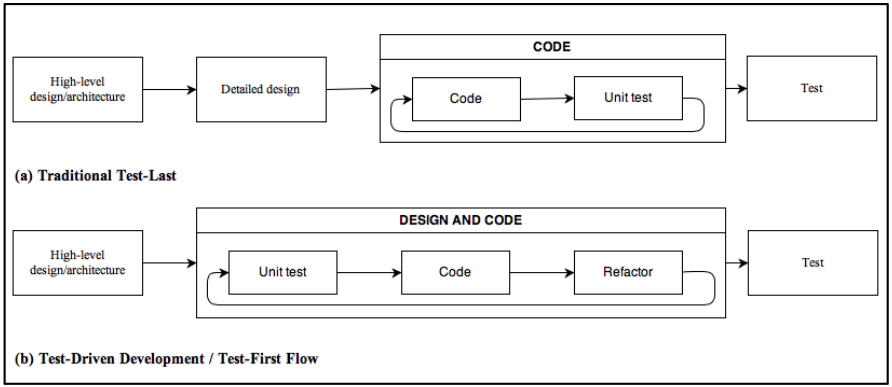
\includegraphics[width=1\textwidth]{figures/mapa-tdd.png}
\caption{Model of Janzen and Saiedian (2008) - Traditional Development vs. TDD}
\label{fig:Traditional Development vs. TDD}
\end{figure}

La figura \ref{fig:Traditional Development vs. TDD} muestra la secuencia de los procesos según \emph{Test-Driven Development} (a) en contraposición con la secuencia tradicional (b).

En base a la metodología seguida, los comentarios dentro del código son esenciales para una buena refactorización de este, permitiendo que sea legible. Como fue explicado, debido al ciclo continuo de prueba, codificación y refactorización es necesaria una rápida comprensión del algoritmo y su funcionalidad. Esta secuencia cíclica facilita reescribir el código de una mejor forma, optimizando no solo el funcionamiento de este si no que eliminando bloques innecesario o duplicado.

Por otro lado, una de las desventajas de emplear \emph{TDD} es que debido a su lógica de diseño emergente carece de un esquema de diseño detallado del sistema completo, que podría ser obtenido con otras metodologías, como, por ejemplo, un enfoque de diseño orientado a objetos (\emph{OOD}).  Para el caso particular de \emph{Gerprin}, no es un punto crucial, debido a que el sistema fue desarrollado con anterioridad y se conocen las interacciones entre los módulos y las funciones que los componen de sobremanera.

\section{Definición de actividades}

El ciclo de vida de un proyecto desarrollado empleando XP está compuesto de seis fases\footnote{http://www.cyta.com.ar/ta0502/v5n2a1.htm}:  

\begin{enumerate}
	\item Exploración
	\item Planificación de las entregas
	\item Iteraciones
	\item Integración y pruebas
	\item Aceptación y entrega
	\item Muerte del proyecto
\end{enumerate}

\subsection{Exploración}

Exploración es la actividad inicial del ciclo de vida del desarrollo de un proyecto empleando \emph{XP} como metodología. Consiste en la realización de las primeras interacciones con el proyecto, tomando conocimiento en líneas generales de las historias de usuario del \emph{software} a desarrollar. 

Es importante en esta etapa definir las herramientas, metodologías, canales de comunicación y \emph{framework} que se utilizaran, además, realizar un primer acercamiento de estas al equipo de trabajo, para familiarizarse con su uso.

\subsection{Planificación de las entregas}

En la etapa de planificación de la entrega se deben definir las prioridades de las historias de usuario y el esfuerzo que debe ser empleado en el desarrollo de dicha historia. Lo anterior con el objetivo de determinar el orden y contenido de los entregables.

Para lo anterior se debe elaborar un informe con las historias de usuario que serán desarrolladas en cada entregable y la estimación del tiempo que tardará en ser completado. El documento debe definir la fecha de finalización de cada una de las iteraciones programadas separadas en plazos de no más de tres semanas. 

Esta etapa se debe repetir antes de cada iteración para definir el contenido del siguiente entregable y corregir, de ser necesario, las estimaciones realizadas en iteraciones anteriores.

Con el fin de obtener una retroalimentación del tiempo de trabajo y poder corregir a tiempo problemas de atraso que se estén produciendo. Se empleará un sistema de puntaje para medir el tiempo de desarrollo de las historias donde un punto equivale a una semana de trabajo de una persona. De este modo cada historia tiene un estimado de trabajo y el valor real de trabajo realizado y se busca que dichos valores sean lo más similar posible.

\subsection{Iteraciones}

Las iteraciones corresponden a varias entregas que se realizan de forma periódica basadas en el documento generado en la etapa anterior.

En la primera iteración se debe realizar un diseño de la arquitectura del sistema, definiendo a grandes rasgos la relación entre las partes que componen el sistema. Lo anterior se logra realizando un breve análisis de las historias de usuario que fuercen el uso de una arquitectura especifica. 

Debido a que la lógica de trabajo se basa en diseño emergente, no es necesario un gran detalle en el diseño. Se debe considerar que dicho diseño puede verse afectado por futuras decisiones en el desarrollo.

En esta etapa se adopta el flujo de trabajo de \emph{TDD}, donde antes de comenzar los trabajos de programación se escriben las pruebas unitarias que deben ser aprobadas por los distintos procesos a desarrollar. Dichas pruebas deben ser realizadas en paralelo a la codificación del programa, de este modo, cada prueba da lugar a una refactorización del código y permite que el diseño emerja desde la optimización del código.

Para comprender de una mejor forma esta lógica de trabajo se debe entender que cada prueba que dé a conocer un error del programa es una prueba exitosa, esto debido a que nos permite conocer los errores antes de que estos pacen al proceso de producción. 

\subsection{Integración y pruebas}

La etapa de Integración y pruebas consiste en la instalación de la aplicación en su ubicación final, donde se realizarán pruebas de integración que permiten comprobar que las configuraciones y relaciones entre las partes del sistema funciones correctamente. 

Junto con lo anterior se debe considerar nuevas funcionalidades para la aplicación que no fueron incluidos en las fases anteriores y que son deseables para nuevas versiones.

\subsection{Aceptación y entrega}

Para esta etapa la aplicación debe ser entregada mientras se encuentra en los servidores de producción, con el objetivo de resolver situaciones que presentaron problemas en las pruebas de integración y desarrollar las funcionalidades que fueron solicitadas en la etapa anterior. 

\subsection{Muerte del proyecto}

Debido a que el proyecto no recibirá más cambios, en esta etapa se debe desarrollar un manual de usuario explicando las funcionalidades del sistema que contenga el propósito de cada función, como usarlas correctamente, los valores configurables, su significado y las restricciones de estos.

Además, un documento de diseño de la arquitectura final del sistema con el propósito de documentar el funcionamiento del sistema en caso de futuras mejoras. 

\section{Productos de Trabajo}

El manifiesto ágil, en el segundo elemento que se ha aprendido a valorar dice “Software funcionando sobre documentación extensiva”. Debido a esto los productos de trabajo generados por cada una de las etapas van enfocadas a un software funcional más que a la documentación.

Sin embargo, el mismo manifiesta concluye “aunque valoramos los elementos de la derecha (documentación), valoramos más los de la izquierda (código funcionando)”. Los productos de trabajo que no corresponden a código funcional, es decir, corresponden a documentos, planes de trabajo, manuales o especificaciones deben encontrarse en proporción al trabajo a realizar.

A continuación, se detallan los productos de trabajo que deben ser generados:

\begin{enumerate}
	\item Especificación de Requerimientos
	\item Planificación de proyecto
	\item Plan de pruebas
	\item Especificación del Sistema
	\item Plan de Aseguramiento de Calidad (\emph{SQA})
	\item Manual de usuario
\end{enumerate}

\subsection{Especificación de Requerimientos}

Para comprender de mejor forma el sistema que se busca construir, es necesario realizar un proceso de documentación esquemática de los requerimientos que forman parte del sistema.

La especificación de requerimiento es un documento que mediante la declaración y definición de los requerimientos funcionales y no funcionales del sistema describe el comportamiento completo de este.

Basado en [BE -11], el siguiente esquema muestra el índice de contenidos del documento. 

\vspace{10mm}
\begin{framed}
     \begin{enumerate}
		\item \textbf{Introducción}
		\begin{enumerate}
			\item Proósito del documento
			\item Alcance del producto
			\item Definiciones, acrónimos y abreviaturas
			\item Referencias
			\item Descripción del resto del documento
		\end{enumerate}
		\item \textbf{Descripción general}
		\begin{enumerate}
			\item Perspectiva del producto
			\item Funciones del producto
			\item Características del usuario
			\item Restricciones generales
			\item Suposiciones y depencencias
		\end{enumerate}		
		\item \textbf{Requerimientos Especificos}

		Incluye los requerimientos funcionales, no funcionales y de interfaz. Obviamente ésta es la parte más sustancial del documento, pero debido a la amplia variedad en la práctica organizacional, no es apropiado definir una estructura estándar para esta sección. Los requerimientos pueden documentar las interfaces externas, describir la funcionalidad y el rendimiento del sistema, especificar los requerimientos lógicos de la base de datos, las restricciones de diseño, las propiedades emergentes del sistema y las características de calidad.
		\item \textbf{Apéndice}
		\item \textbf{Índice}
	\end{enumerate}
\end{framed}

\subsection{Planificación de proyecto}
Antes de comenzar a escribir código, es necesario planear las distintas entregas y el contenido de estas. El documento debe contener las historias de usuarios que serán incluidas en cada iteración y las fechas de entrega de cada una de estas.

Para lograr establecer una correcta planificación de las iteraciones, se deben escribir todas las historias de usuario del sistema, para luego valorarlas en termino de complejidad e importancia, de este modo se establece la ruta crítica en las actividades a realizar. 

Se debe notar que debido a las características del trabajo de desarrollo de \emph{software} es necesario ser flexible sobre el contenido de cada entrega, considerando cambios solicitados por el cliente, corregir errores detectados en iteraciones anteriores, entre otras actividades que pueden ser incluidas en iteraciones futuras. Debido a esto es necesario contemplar modificar la planificación con cada nueva iteración.

El esquema muestra el índice de contenido del producto de trabajo, basado en [BE -11]

\begin{framed}
     \begin{enumerate}
		\item \textbf{Introducción}
		\begin{enumerate}
			\item Objetivo
			\item Alcance 
		\end{enumerate}
		\item \textbf{Estimación de esfuerzo y duración}
		\begin{enumerate}
			\item Estimación de esfuerzo
		\end{enumerate}		
		\item \textbf{Organización del Proyecto}

		Describe la forma en que el equipo de desarrollo está organizado, la gente involucraday sus roles.
		\item \textbf{Planificación}

		Descomposicion detallada de las actividades. Señala el \emph{hardware} y \emph{software} de ayuda requeridos para llevar a cabo el desarrollo. Describe la division del proyecto en actividades e identifica hitos asociados a cada actividad.
		\item \textbf{Estrategia del seguimiento}
		\item \textbf{Interfaz externa al proyecto}
		\item \textbf{Identificación y análisis de los riesgos}
	\end{enumerate}
\end{framed}

\subsection{Plan de pruebas}

Uno de los ejes fundamentales al trabajar bajo \emph{TDD} son las pruebas constantes que deben ser realizadas para asegurar un correcto funcionamiento. El plan de pruebas, al igual que la planificación de iteraciones, es un documento que sufrirá modificaciones y será escrito a lo largo del desarrollo del proyecto.

Ante de comenzar la labor de codificación de cada iteración, se deben escribir las distintas pruebas que confirmaran la integración y funcionamiento correcto de cada entregable. 

Antes de desarrollar cualquier función se deben establecer las siguientes pruebas. 

\begin{description}
	\item[Pruebas unitarias:]\hfill

	Son pruebas que aseguran el correcto funcionamiento de una unidad específica del sistema. 

	\item[Pruebas de integración:]\hfill

	Pruebas que comprueban que la correcta integración de todos los elementos unitarios que componen el sistema.

	\item[Pruebas de aceptación:]\hfill

	Las pruebas de aceptación son realizadas en la última iteración y prueban el sistema completo antes de ser instalado en ambiente productivo.

	\item[Pruebas de sistema:]\hfill

	Las pruebas de sistema realizan una comparación entre los objetivos originales del sistema, aquellos planteados en la toma de requisitos, y los procesos, actividades y rutinas del sistema desarrollado.
\end{description}

El esquema muestra el índice de contenido del producto de trabajo, basado en [BE -11]

\begin{framed}
     \begin{enumerate}
		\item \textbf{Introducción}
		\begin{enumerate}
			\item Objetivo
			\item Alcance 
		\end{enumerate}
		\item \textbf{Definición de elementos a probar}	
		\item \textbf{Definición de la estrategia a utilizar}

		Describe los recursos a emplear. Especificacion de técnica que se usará. Herramientas utilizadas. Criterio indicador de éxito de las pruebas.
		\item \textbf{Equipo de pruebas}
	\end{enumerate}
\end{framed}

\subsection{Especificación del Sistema}

Debido a que la labor de \emph{software} es un trabajo realizado en equipo, es necesario dejar plasmada la arquitectura del sistema y explicar a grandes rasgos el funcionamiento de los distintos procesos. Esto con el objetivo de ayudar a futuros desarrolladores que realicen labores de mantención o actualizaciones al sistema.

Las especificaciones del sistema deben contener la arquitectura y descripción de las funciones que componen cada una de las distintas partes.

El esquema muestra el índice de contenido del producto de trabajo, basado en [BE -11]

\begin{framed}
     \begin{enumerate}
		\item \textbf{Introducción}
		\begin{enumerate}
			\item Objetivo
			\item Alcance 
		\end{enumerate}
		\item \textbf{Identificación de necesidades}
		Describe el análisis técnico y económico. Se debe ralizar un análisis para evaluar su visibilidad	
		\item \textbf{clasificación de funciones}
		\begin{enumerate}
			\item Funciones de \emph{Software}
			\item Funciones de \emph{Hardware}
			\item Funciones del personal
		\end{enumerate}		
		\item \textbf{Restricciones del sistema}
		\item \textbf{Esquema relacional del sistema}
	\end{enumerate}
\end{framed}

\subsection{Plan de Aseguramiento de Calidad (\emph{SQA})}
Es necesario asegurar la calidad del \emph{software} desarrollado, asegurando el cumplimiento de los distintos requerimientos desarrollados.

El documento es un resumen de las actividades desarrolladas y la confirmación de su cumplimiento, mediante la validación de los resultados. En el plan de aseguramiento de calidad se debe especificar los resultados obtenidos y compararlos con los resultados esperados.

El documento debe contener las modificaciones, revisiones y demás actividades que se realizaron en caso de no obtener los resultados esperados.

El esquema muestra el índice de contenido del producto de trabajo, basado en [BE -11]

\begin{framed}
    \begin{enumerate}
		\item \textbf{Introducción}
		\begin{enumerate}
			\item Objetivo
			\item Alcance
			\item Definiciones
			\item Resumen
		\end{enumerate}
		\item \textbf{Gestión SQA}
		\begin{enumerate}
			\item Actividades
			\item Resultado obtenido en las actividades
			\item Revisiones y auditorías
		\end{enumerate}
	\end{enumerate}
\end{framed}

\subsection{Manual de usuario}
Final mente el manual de usuario es un documento que tiene como objetivo describir el funcionamiento del sistema al usuario final. 

El documento debe explicar el funcionamiento y propósito de cada una de las historias de usuario que componen el sistema. De este modo el usuario comprende el propósito y uso correcto de \emph{software} y \emph{hardware}.

En la sección final del documento debe incluir la forma de contacto al área de soporte, con el finde aclarar las consultas más específicas.

El esquema muestra el índice de contenido del producto de trabajo, basado en [BE -11]

\begin{framed}
     \begin{enumerate}
		\item \textbf{Prefacio}
		\begin{enumerate}
			\item Resumen
			\item Cómo usar el manual
		\end{enumerate}
		\item \textbf{Índice}
		\item \textbf{Modelo del sistema}
		\item \textbf{Funciones principales del sistema}
		\item \textbf{Sección de preguntas}
		\begin{enumerate}
			\item pregunta frecuentes 
		\end{enumerate}
		\item \textbf{Contáctenos}
	\end{enumerate}
\end{framed}

\section{Hitos del desarrollo (Atributos de Calidad)}

\subsection{Por actividades}

\begin{table}[H]
    \caption[Hitos del desarrollo por actividades.] {Hitos del desarrollo por actividades.}
    \label{tbl:Objetivos Cuantificales y atributos de calidad por actividades}
    \begin{tabular}{|p{.6\textwidth}|p{.34\textwidth}|}
        \hline
        \textbf{Actividad} &  \textbf{Atributo}\\
    	\hline
    	\hline
    	Exploración & Se deben respetar los plazos de entrega del proyecto. Fiabilidad \\ \hline
    	Planificación de las entregas & Debe ser fiable, respetando los plazos y fechas definidos junto al cliente y al mismo tiempo, debe ser flexible, permitiendo modificaciones y actualizaciones.
		El cliente debe estar de acuerdo con las fechas de entrega y el contenido de estas. \\ \hline
    	Iteraciones & El trabajo realizado en esta etapa, debe ser eficiente y cumplir en un 100\% con lo establecido en las actividades anteriores. El producto debe ser fiable, mantenible, multiplataforma y adaptable. Respecto a los entregables, el cliente debe aceptar el 100\% de las funcionalidades del sistema. \\ \hline
    	Integración y pruebas & Al igual que en la etapa anterior, el trabajo debe ser eficiente, además, debe ser mantenible y el producto debe ser fiable. Se deben corregir el 100\% de las fallas encontradas en la actividad anterior. \\ \hline
    	Aceptación y entrega & El trabajo debe ser adaptable y escalable. El proceso de instalación debe ser eficiente y fiable. EN esta etapa el 100\% de las funcionalidades del sistema deben ser aceptadas por el cliente. \\ \hline
    	Muerte del proyecto & El 100\% de las funciones deben encontrarse documentadas, tanto en lenguaje técnico como en lenguaje común. En caso de encontrar fallas estas deben ser solucionadas en un plazo máximo de 8 horas hábiles. Las tareas realizadas en esta etapa deben ser mantenibles, eficientes y adaptables.  \\ 
        \hline
    \end{tabular}
\end{table}

\subsection{Por producto}

\begin{table}[H]
    \caption[Hitos del desarrollo por productos.] {Hitos del desarrollo por productos.}
    \label{tbl:Objetivos Cuantificales y atributos de calidad por productos}
    \begin{tabular}{|p{.6\textwidth}|p{.34\textwidth}|}
        \hline
        \textbf{Producto} &  \textbf{Atributo}\\
    	\hline
    	\hline
    	Especificación de Requerimientos  & El documento debe contemplar el 100\% de los requerimientos acordados con el cliente. Debe ser fiable y escalable. \\ \hline
    	Planificación de proyecto & Mantenible y adaptable. Debe contener el 100\% de las actividades a realizadas. \\ \hline
    	Plan de pruebas & Mantenible, adaptable y fiable. Debe contener pruebas unitarias, de integración, compatibilidad y aceptación. \\ \hline
    	Especificación del Sistema & Fiable, adaptable y mantenible. Debe ser aprobado en un 100\% por el equipo de desarrollo y el cliente. \\ \hline
    	Plan de Aseguramiento de Calidad (SQA)  & Mantenible, adaptable, fiable, seguro, escalable. Debe comprobar en un 100\% la calidad del sistema.  \\ \hline
    	Manual de usuario & Fiable. Debe ser comprensible en un 100\% por el cliente, debe contener un índice y no superar la extensión de 40 paginas  \\ 
        \hline
    \end{tabular}
\end{table}

\section{Puntos de revisión}
Los puntos de revisión en cada una de las distintas etapas son los siguientes 
\begin{enumerate}
	\item Exploración
	\begin{enumerate}
		\item Revisión y aprobación de las especificaciones de requerimientos
		\item Revisión y aprobación de las historias de usuario (preliminar)
	\end{enumerate}
	\item Planificación de las entregas
	\begin{enumerate}
		\item Revisión y aprobación de la actualización de las historias de usuario (se actualiza en cada iteración)
		\item Revisión y aprobación de la actualización de la planificación de la Iteración (se actualiza en cada iteración)
		\item Revisión y aprobación de plan de pruebas unitarias, de integración y de sistema (se actualiza en cada iteración)
	\end{enumerate} 
	\item Iteraciones
	\begin{enumerate}
		\item Revisión y aprobación de la actualización del modelo del modelo entidad relación
		\item Revisión y aprobación del código (se actualiza en cada iteración)
		\item Revisión y aprobación de la actualización del documento de especificaciones del sistema (se actualiza en cada iteración)
		\item Revisión y aprobación de las pruebas unitarias, de aceptación y de integración.
		\item Revisión y aprobación de documentación de resultado asociado a las pruebas unitarias, de aceptación y de integración. 
		\item Revisión de la actualización Plan de Aseguramiento de Calidad (se actualiza en cada iteración)
	\end{enumerate} 	
	\item Integración y pruebas
	\begin{enumerate} 
		\item Revisión y aprobación del proceso de integración.
		\item Revisión y aprobación de la prueba de integración. 
		\item Revisión y aprobación de documentación de resultado asociado a las pruebas de integración. 
		\item Revisión y aprobación del documento de especificaciones del sistema
		\item Revisión de la actualización Plan de Aseguramiento de Calidad (se actualiza en cada iteración).
	\end{enumerate}
	\item Aceptación y entrega.
	\begin{enumerate} 
		\item Revisión y aprobación de modificaciones en el código del sistema.
		\item Revisión y aprobación de las especificaciones del sistema asociada a las modificaciones.
		\item Revisión de la actualización Plan de Aseguramiento de Calidad.
	\end{enumerate}
	\item Muerte del proyecto.
	\begin{enumerate}
		\item Revisión y aprobación del manual de usuario
		\item Revisión de la actualización Plan de Aseguramiento de Calidad.
	\end{enumerate}
\end{enumerate}
%!TEX root = ../memoria.tex

\chapter{Gestion de calidad}

\section{Equipo de trabajo}

A continuación, se presenta un esquema que muestra la estructura del equipo de trabajo basado en \citep{web00}
\begin{figure}[ht!]
\centering
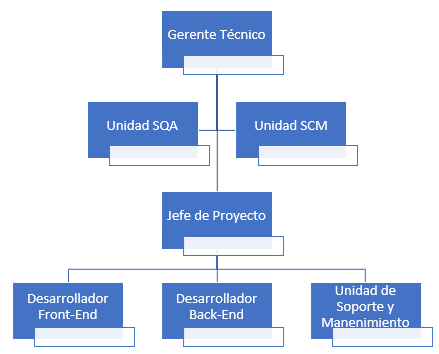
\includegraphics[width=.7\textwidth]{figures/equipo-trabajo.png}
\caption{Equipo de trabajo}
\label{fig:Equipo de trabajo}
\end{figure}

Según Don Wells, autor de las reglas de \emph{Extreme Programming},  el equipo debe tener dos características transversales:

	\begin{itemize}
		\item 
		 \textbf{Coraje}: Se debe ser sincero respecto al progreso y plazos del proyecto. Los trabajadores forman parte de un equipo, por lo que no deben temer a nada
		\item
		 \textbf{Respeto}: Se debe respetar a todos los miembros del equipo y clientes. Cada trabajador realiza un aporte valioso al equipo, por lo que debe ser respetado.
	\end{itemize}

\section{Recursos}
\subsection{Personal}
\subsubsection{Gerente Técnico}

Las responsabilidades del gerente técnico son:

	\begin{itemize}
		\item 
		 Establecer y seleccionar el lineamiento de un programa de calidad para el desarrollo de \emph{software}.
		\item
		 Revisar y aprobar el plan de \emph{SQA} para cada proyecto. 
		 \item
		 Facilitar al equipo los medios para la realización de las actividades asociadas al plan de \emph{SQA}.
		 \item 
		 Monitorear las actividades de \emph{SQA}.
	\end{itemize}

\subsubsection{Unidad \emph{SQA}}

Son los encargados de generar el plan de aseguramiento de calidad que incluyen el aseguramiento de calidad de entregables y documentación. Si bien, son los encargados de realizar el plan de calidad, no son encargados de velar por la realización de las actividades asociadas al plan o de prácticas, procesos y procedimientos. Dicha responsabilidad recae en el jefe de proyecto y encargados de cada área.

Las responsabilidades de la unidad de \emph{SQA} son: 

	\begin{itemize}
		\item 
		 Establecer los estándares de calidad.
		\item
		 Observar, participar y verificar que las revisiones de calidad se realicen correctamente. 
		 \item
		Velar por la correcta realización de las distintas pruebas y procedimientos establecidos de acuerdo con el plan de pruebas.
		 \item 
		Crear un plan de identificación de defectos para el proceso de desarrollo y apoyar a áreas de gestión en perfeccionar estos.
	\end{itemize}

\subsubsection{Unidad \emph{SCM}}

La unidad de Gestión de Configuración del \emph{Software} es la encargada de mantener la integridad del producto a lo largo de todo el desarrollo del proyecto, mediante un control de cambios adecuado para el desarrollo.

Las responsabilidades de \emph{SCM} asociadas a \emph{SQA} son: 

	\begin{itemize}
		\item 
		Revisar y comentar el plan de \emph{SQA} para el proyecto. 
		\item
		Implementar las actividades de calidad de acuerdo con el plan de \emph{SQA}. 
		 \item
		Resolver los problemas detectados por \emph{SQA} relacionados con \emph{SCM}.
		 \item 
		Implementar las prácticas, procesos y procedimientos definidos en el plan de \emph{SCM} y en otros planes o documentos complementarios.
	\end{itemize}

\subsubsection{Jefe de Proyecto}

Las responsabilidades del jefe de proyecto son:

\begin{itemize}
		\item 
		Establecer un programa de calidad para el proyecto de desarrollo de \emph{software} de acuerdo con las políticas organizacionales.
		\item
		Identificar las actividades de \emph{SQA} requeridas para el proyecto.
		\item
		Revisar y aprobar el plan de \emph{SQA} para el proyecto.
		\item 
		Identificar los participantes de las actividades de \emph{SQA}.
		\item
		Implementar las actividades de \emph{SQA} de acuerdo con el plan.
		\item
		Monitorear las actividades de \emph{SQA} planificadas en el plan.
		\item
		Identificar los factores de calidad para la implementación del software.
		\item
		Identificar, desarrollar y mantener la documentación del proyecto. 
	\end{itemize}

\subsubsection{Desarrolladores \emph{Front-End}, Desarrolladores \emph{Back-End} y Soporte y mantenimiento}

El área de soporte y mantenimiento es el encargado de realizar correcciones y solucionar problemas relacionados con el correcto funcionamiento del sistema una vez este se encuentre en ambientes productivos. Esto se traduce en identificar causas de errores mediante el registro de actividades de la aplicación y dar soporte a consultas del cliente.

Por otro lado, el área de desarrollo se divide en desarrolladores \emph{Front-End} y \emph{Back-End} que hace referencia a la capa del sistema sobre la cual realizan su trabajo de desarrollo. 

El desarrollador \emph{Front-End} trabaja sobre la capa de presentación de datos, es decir, la que interactúa directamente con el usuario. Mientras el desarrollador \emph{Back-End} trabaja sobre la capa de acceso de datos que se encarga de procesar la información proveniente de la capa de presentación

Sus responsabilidades con \emph{SQA} son: 

	\begin{itemize}
		\item
		Revisar y entregar sus observaciones sobre el plan de \emph{SQA} para el proyecto.
		\item
		Implementar las actividades de \emph{SQA} de acuerdo con el plan.
		\item
		Participar de la solución de los problemas detectados por las actividades de \emph{SQA} que sean de su competencia.
		\item
		Implementar las prácticas, procesos y procedimientos definidos en el plan de proyecto y en otros planes o documentos complementarios.
	\end{itemize}

\subsection{Infraestructura}

Además de los recursos humanos necesarios para el correcto desarrollo del sistema y la Realización de las actividades de \emph{SQA}.

\subsubsection{Oficina}

Es necesaria una oficina que cuente con áreas de trabajo y salas de reuniones. Respecto a las áreas de trabajo estas deben contar con escritorios y sillas ergonómicas recomendadas para trabajo de escritorio que cuenten con altura variable y soporte para brazos y espalda. Los escritorios deben contar con un largo no inferior a un metro y un ancho no inferior a 70 cm. 

Respecto a las oficinas de reuniones, esta debe contar con un televisor que permita conexión a un equipo (\emph{notebook} o dispositivo móvil) o en su defecto un proyector.
Es necesario que la oficina cuente con los servicios básicos como luz y agua potable. Finalmente es necesario contar con una conexión de internet no menor de 30 Mbps.

\subsubsection{Equipamiento de trabajo}

Es necesario contar con un mínimo de 5 equipos de trabajo enfocados en el desarrollo.

	\begin{itemize}
		\item 
		\textbf{Procesador}: Intel Core i7-7700.
		\item 
		\textbf{Memoria}: 12GB DDR4 (2400 MHz).
		\item 
		\textbf{Almacenamiento}: Unidad SSD 240GB Lectura 540 MB/s Escritura 465 MB/s.
		\item 
		\textbf{Pantalla}: Dos pantallas de mínimo 17”.
	\end{itemize}

Además, es necesario  3 equipos Laptop para uso administrativo. 

	\begin{itemize}
		\item 
		\textbf{Procesador}: Intel Core i5 7200U.
		\item 
		\textbf{Memoria}: 8GB DDR4 (2400 MHz).
		\item 
		\textbf{Almacenamiento}: HDD 1TB (5400rpm).
	\end{itemize}

\subsection{Actividades}

El área de \emph{SQA}, con el objetivo de asegurar la calidad de forma continua, se debe encargar de varias actividades a lo largo del proceso de desarrollo de \emph{Gerprin}. Es importante que \emph{SQA} realice las definiciones de estándares, revisión de productos y procesos, pruebas y análisis de defectos hasta la entrega exitosa de las últimas modificaciones y posteriores documentaciones del sistema. Para esto debe trabajar en conjunto con las áreas de desarrollo, tanto \emph{Front-End}, \emph{Back-End}, unidades de soporte, mantenimiento e implantación.

Las siguientes actividades se encuentran basadas en Herramientas específicas para el grupo de \emph{SQA} \citep{web00}.

\subsubsection{Evaluación de la selección de los productos de trabajo}

El \emph{SQA} debe asistir al jefe de proyectos en la elaboración de los estándares y guías aplicables que conforman los distintos artefactos necesarios para la planificación inicial del proyecto. Entre los elementos que deben ser considerados son herramientas por utilizar, diseño preliminar y \emph{mockup} de la interfaz del sistema, entre otros.

\subsubsection{Evaluación de las herramientas} 

En esta actividad el \emph{SQA} tiene la responsabilidad de evaluar las herramientas que serán empleadas para el desarrollo del sistema, considerando herramientas para pruebas, evaluaciones de rendimiento de la aplicación y herramientas de administración de proyectos.

Por otro lado, junto con el jefe de proyecto deben ser decididas las herramientas empleadas directamente en el proceso de desarrollo como \emph{frameworks}, herramientas de despliegue de aplicaciones, entre otros.

\subsubsection{Evaluación de la planificación y el monitoreo del proyecto}

\emph{SQA} es responsable de la elaboración del plan de aseguramiento de calidad, la elaboración e identificación de guías y estándares que puedan ser aplicados a las iteraciones y entregables.

\subsubsection{Evaluación de la especificación de requerimientos}

Respecto a las especificaciones de requerimiento \emph{SQA} debe realizar las siguientes actividades:

	\begin{itemize}
		\item 
		Verificar que se cumplan correctamente las actividades y procesos de la fase de exploración.
		\item
		Garantizar que se revisaron adecuadamente los entregables (especificación del sistema y de requerimientos) de la fase de exploración. 
		\item
		Asegurar la inclusión de la corrección de los entregables según las observaciones realizadas en el proceso de revisión. 
		\item
		Corroborar que estén expresados y documentados los requerimientos funcionales, técnicos, operacionales y de interfaz, de manera tal que puedan ser verificados en el producto final.
	\end{itemize}

\subsubsection{Evaluación del diseño}

\emph{SQA} es responsable de:

	\begin{itemize}
		\item 
		Garantizar que se revisaron adecuadamente los entregables (diseño preliminar, diseño detallado, plan de pruebas, especificación de casos y procedimientos de prueba) de la fase de planificación de las entregas e iteraciones.
		\item
		Asegurar la inclusión de la corrección de los entregables según las observaciones realizadas en el proceso de revisión.
	\end{itemize}
	
\subsubsection{Evaluación de la implementación y de la prueba de unidad}

\emph{SQA} debe:

	\begin{itemize}
		\item 
		Garantizar que el proceso de codificación, las revisiones asociadas y la prueba de unidad sean conducidos de acuerdo a lo señalado en el plan de pruebas.
		\item
		Asegurar la inclusión de la corrección de los entregables según las observaciones realizadas en el proceso de revisión.
		\item
		Verificar la implementación de las acciones correctivas derivadas de la prueba de unidad.
		\item
		Comprobar la utilización de la especificación de procedimientos y casos de prueba durante la prueba de unidad. 
		\item
		Corroborar la documentación del código y de los resultados de la prueba de unidad.
	\end{itemize}

\subsubsection{Evaluación de la integración y prueba}

\emph{SQA} es responsable de:

	\begin{itemize}
		\item 
		Verificar que el proceso de integración y las actividades de prueba sean realizadas conforme al plan de proyecto, el diseño, el plan de prueba y los estándares y procedimientos establecidos.
		\item
		Asegurar que la prueba de integración fue completada satisfactoriamente, que sus resultados fueron registrados y divulgados y que las acciones correctivas derivadas de ella fueron implementadas.
		\item	
		Corroborara el desarrollo adecuado de las pruebas de aceptación y del sistema.
		\item
		Monitorear las actividades de prueba y certificar sus resultados.
		\item
		Revisar las pruebas.
	\end{itemize}

\subsubsection{Evaluación del producto antes de su liberación}

Se deben realizar las evaluaciones del producto terminado y la documentación. Para esto es necesario que el área de \emph{SQA} sea participe de las auditorias funcionales y físicas. 

\subsubsection{Evaluación del proceso de revisión}

\emph{SQA} es responsable de garantizar que todos los entregables sean revisados y corregidos en caso de ser necesario y analizar los problemas encontrados de una forma sistémica, identificando causas, impactos y frecuencia de ocurrencia.

\subsubsection{Evaluación de las acciones correctivas}

\emph{SQA} es responsable de establecer acciones preventivas y monitorear que estas sean implementadas de forma correcta. 

\subsubsection{Evaluación del proceso de \emph{SCM}}

\emph{SQA} debe:

\begin{itemize}
		\item 
		Revisar el plan de \emph{SCM}.
		\item 
		Asegurar la correcta identificación de los ítems de configuración.
		\item 
		Garantizar un adecuado control de cambios.
		\item 
		Corroborar que la contabilidad del estado de la configuración sea preparada oportunamente y que refleje la situación real de los ítems de configuración en relación con el proyecto.
		\item 
		Comprobar la adherencia de las actividades de \emph{SCM} al plan de \emph{SCM}.
		\item 
		Verificar el correcto funcionamiento de la librería del \emph{software}.
	\end{itemize}

\subsubsection{Verificar la implementación de los procesos}

\emph{SQA} debe velar por la correcta implementación y cumplimiento de estándares y procesos definidos en las especificaciones de requisitos y planificación de iteraciones.

\subsubsection{Establecer las auditorías}

\emph{SQA} es responsable en la institución por el desarrollo de las auditorías internas. Por lo tanto, debe gestionarlas de ser preciso.

Además, es su responsabilidad participar en la auditoría física y funcional.

\subsubsection{Responsabilidades}

El área de \emph{SQA} es responsable de revisar que los productos de trabajo se adecuen a los estándares, procedimientos y al plan de proyecto, además de dar seguimiento a las actividades realizadas a lo largo del desarrollo del proyecto. Todo lo anteriormente observado debe ser informado al jefe de proyecto y de ser necesario al jefe de proyecto.

En la siguiente tabla se adjunta la matriz de responsabilidades \citep{web00}.

\begin{table}[H]
    \caption[Responsabilidades por actividades.] {Responsabilidades por actividades.}
    \label{tbl:responsabilidades por actividades}
    \begin{tabular}{|p{.2\textwidth}|p{.035\textwidth}|p{.03\textwidth}|p{.05\textwidth}|p{.055\textwidth}|p{.09\textwidth}|p{.11\textwidth}|p{.1\textwidth}|p{.07\textwidth}|}
        \hline
        \textbf{Actividad} &  \textbf{GT} & \textbf{JP} & \textbf{SQA} & \textbf{SCM} & \textbf{Analista} & \textbf{Front-End} & \textbf{Back-End} & \textbf{Tester}\\
    	\hline
    	\hline
    	Evaluación	de la selección los productos de trabajo. & X & X & X & X & X & & & \\ \hline
    	Evaluación de las herramientas & X & X & X & & & & & \\ \hline
    	Evaluación de la planificación y el monitoreo del proyecto & X & X & X & X & & & & \\ \hline
    	Evaluación de la especificación de requerimientos & X & X & X & & X & X & X & X \\ \hline
    	Evaluación del diseño & X & X & X & & X & X & X & X \\ \hline
    	Evaluación de la implementación y de la prueba de unidad & & & X & & & X & X & X \\ \hline
    	Evaluación de la integración y prueba & & & X & & & X & X & X \\ \hline
    	Evaluación del producto antes de su liberación & & X & X & & X & X & X & X \\ \hline
    	Evaluación del proceso de revisión & & X & X & & & & & \\ \hline
    	Evaluación de las acciones correctivas & X & X & X & X & & & & \\ \hline
    	Evaluación del proceso de \emph{SCM} & X & X & X & X & & & & \\ \hline
    	Verificar la implementación de los procesos & & X & X & & & & & \\ \hline
    	Establecer las auditorías & & X & X & X & & & & \\ \hline
    	
    \end{tabular}
\end{table}















	




%!TEX root = ../memoria.tex

\chapter{Herramientas, técnicas y metodologías}

En el presente capitulo se identifican técnicas y herramientas que serán implementadas por el equipo de SQA para un aseguramiento de calidad eficiente y efectivo.

Para actividades de IT existen muchas herramientas y técnicas que permiten disminuir la cantidad de errores y facilitan la correcta ejecución de distintas actividades del desarrollo del software. A continuación, se procederá a indicar actividades que garanticen el progreso de la labor de SQA hacia un cumplimiento de los objetivos de este.

\section{Técnicas}

Una de las técnicas principales a emplear en el desarrollo del software corresponde a TDD, que fue descrita anteriormente (3.1). Esta técnica no solo permite reducir los errores de cada release, también permite una detección temprana de estos.

\section{Herramientas}

Serán empleadas distintas herramientas para las actividades de SQA a continuación se detallan estas y el objetivo de su uso.

\begin{itemize}
	\item 
		El canal de comunicación formar será mediante correo electrónico. Adicionalmente se empleará Discord como un canal de comunicación secundario para realizar conversaciones de carácter inmediato.
	\item
		Se emplearán procesadores de texto online para la documentación de resultados tales como Microsoft office 365.
	\item
		Para el ingreso, edición, recolección y asignación de los defectos encontrados se empleará ActiveCollab. Además, permite la creación de carta Gantt y asignación de actividades.
	\item
		Para la generación de test automáticos y casos de pruebas se realizará con el software SoapUI.
	\item 
		Para mejorar el uso de un sistema de control de versiones se empleará Git Flow, que permite estandarizar el flujo de trabajo de Git.
\end{itemize}

Finalmente se empleará como IDE de trabajo PyCharm que permite identificar de forma rápida errores comunes de programación como variables no definidas o código duplicado entre otras. 

\section{Revisiones}

Las revisiones son una metodología empleada en SQA, utilizada para la detección temprana de desviaciones y defectos. El objetivo de las revisiones es visibilizar el proceso de desarrollo con el fin de realizar un monitoreo a productos y procesos.

SQA debe velar por la correcta realización y documentación de las revisiones. Adicionalmente es responsable por la correcta asignación, documentación y programación de las actividades que deben ser realizadas al detectar cualquier anomalía en estas.

Basado en \citealp{web00} se procede a describir los participantes y de forma seguida, las etapas que conforman parte del proceso de revisión. 

\subsection{Roles y responsabilidades}

Los actores descritos a continuación deben guiarse por el checklist de la revisión adjunto en anexos. 

\subsubsection{Moderador}

El moderador es el encargado de facilitar todo el proceso de revisión, debe liderar el resto del equipo, coordinar las actividades, trabajar con los jefes de proyecto de otras secciones, preparar las inspecciones coordinando al equipo de trabajo, determinar el alcance la de inspección e informar los productos de las actividades de inspección a jefes de proyecto.

\subsubsection{Autor}

Corresponde al autor del producto a ser inspeccionado. Debe preparar el producto para ser inspeccionado, realizar recomendaciones de personas que participen en el proceso de inspección, explicar el producto a ser inspeccionado, corregir defectos detectados y participar de las acciones correctivas posteriores.

\subsubsection{Presentador}

El presentador es el encargado de presentar el producto de trabajo al resto del equipo encargado de la inspección, debe comprender a cabalidad el producto con el objetivo de guiar al equipo de trabajo en el proceso de inspección. 

\subsubsection{Inspector}

Es el encargado de inspeccionar el producto de trabajo e identificar errores y defectos. Se encarga del proceso de inspección según las instrucciones entregadas por el moderador. 

\subsubsection{Secretario}

Se encarga de realizar el registro de las observaciones, identificando y clasificando los defectos encontrados, participa de la inspección en igualdad al resto del equipo y una vez finalizada la inspección debe leer cada defecto y su clasificación. Adicionalmente se encarga de anotar acciones correctivas y los plazos de estas. 

\subsubsection{Observador}

El rol de observador es opcional. Se encarga de observar y apuntar la información de los participantes del proceso de revisión y del proceso mismo con el objetivo de poder realizar mejora continua a las actividades realizadas. 

\subsection{Etapas de Revisión}

\subsubsection{Planificación}

\paragraph{Objetivo\\}

El objetivo de esta etapa es verificar que el producto se encuentre en condiciones de ser inspeccionado y planificar las actividades para garantizar el éxito de la revisión.

\paragraph{Participantes\\}

Moderador y el autor.

\paragraph{Criterios de entrada}

\begin{enumerate}
	\item 
		El autor señala que el producto de trabajo está listo para la revisión.
	\item
		La existencia de participantes apropiados y con disponibilidad de tiempo.
\end{enumerate}

\paragraph{Actividades}
\begin{enumerate}
	\item 
		Selección de los participantes y asignación de roles.
	\item
		Determinar el tamaño del producto de trabajo por ser revisado.
	\item
		Determinar los criterios que el producto debe satisfacer.
	\item
		Establecer la necesidad de una reunión orientación.
	\item
		Planificar la reunión de orientación y/o la inspección.
	\item
		Preparación y distribución del paquete de revisión a los participantes.
	\item
		Registro del tiempo usado durante la fase de planificación.
\end{enumerate}

\paragraph{Criterios de salida\\}

Cada participante completa satisfactoriamente la checklist de las tareas asignadas a la etapa de planificación. 

\subsubsection{Orientación (opcional)}

\paragraph{Objetivo\\}

El objetivo de esta reunión es instruir a los participantes sobre el producto de trabajo y reconocer el proceso de revisión que se aplicará a dicho producto.

\paragraph{Participantes\\}

Moderador, autor y cualquier otro participante que requiera información sobre el producto o el proceso de revisión.

\paragraph{Criterios de entrada\\}

Los criterios de salida de la etapa de planificación han sido completados satisfactoriamente.

\paragraph{Actividades}

\begin{enumerate}
	\item 
		Descripción general del producto de trabajo sujeto a inspección.
	\item
		Revisar la asignación de roles y el plan para la inspección.
	\item
		Responder cualquier consulta.
\end{enumerate}

\paragraph{Criterios de salida}

\begin{enumerate}
	\item 
		Todos los participantes están preparados para proceder.
	\item
		Todos los participantes están preparados para proceder.
\end{enumerate}

\subsubsection{Preparación}

\paragraph{Objetivo\\}

El objetivo de esta etapa es que cada miembro evalúe el producto de trabajo para detectar defectos, clasifique estos defectos y los documente. 

\paragraph{Participantes\\}

Moderador, presentador y cualquier participante bajo el rol de inspector.

\paragraph{Criterios de entrada\\}

Los criterios de salida de la etapa de planificación y de la orientación han sido completados satisfactoriamente.

\paragraph{Actividades}
\begin{enumerate}
	\item 
		Los inspectores revisan el producto de trabajo y registran los defectos detectados.
	\item
		Clasificar todos los defectos.
	\item
		El presentador se prepara para exponer el producto durante la reunión de inspección.
	\item
		Entrega del informe de revisión.
\end{enumerate}

\paragraph{Criterios de salida}

\begin{enumerate}
	\item 
		Los defectos han sido correctamente documentados. 
	\item
		Todos los participantes están preparados para proceder en la inspección.
	\item
		Cada participante completa satisfactoriamente la checklist de las tareas asignadas a la etapa de preparación.
\end{enumerate}

\subsubsection{Inspección}

\paragraph{Objetivo\\}

Los objetivos de esta etapa son que los participantes lleguen a un consenso respecto de los defectos que afectan al producto de trabajo, decidan si requiere de una revisión adicional, y que discutan y documenten sobre las lecciones aprendidas durante el proceso.

\paragraph{Participantes\\}

Moderador, presentador, autor, inspector(es), secretario y, opcionalmente, un observador.

\paragraph{Criterios de entrada\\}

Todos los participantes pueden participar de la inspección.

\paragraph{Actividades}

\begin{enumerate}
	\item
		Se enuncian los roles, el enfoque y las guías para llevar a cabo la inspección.
	\item
		El presentador describe el producto de trabajo.
	\item		
		Se nombran los defectos globales que afectan la completitud del producto de trabajo.
	\item		
		Se nombran los defectos específicos por ser revisados y registrados.
	\item		
		Los errores de formatos son entregados al autor para acciones correctivas.
	\item
		Asignación de las los defectos no resueltos.
	\item 
		Determinación sobre la necesidad de tiempo adicional. 
	\item
		Emplear la hora adicional para terminar las actividades restantes.
	\item
		Establecer la necesidad de una revisión adicional.
	\item
		Solicitar retroalimentación a los participantes en relación con la inspección.
\end{enumerate}

\paragraph{Criterios de salida}

\begin{enumerate}
	\item
	Los defectos han sido registrados
	\item
	Los defectos no resueltos han sido asignados.
\end{enumerate}

\subsubsection{Rework}

\paragraph{Objetivo\\}

El objetivo de esta etapa es corregir los defectos y resolver aquellos clasificados como no resueltos.

\paragraph{Participantes\\}

Autor.

\paragraph{Criterios de entrada\\}

Los criterios de salida de la etapa de inspección han sido completados satisfactoriamente.

\paragraph{Actividades}

\begin{enumerate}
	\item
		Estimar el tiempo requeridos para resolver los defectos no resueltos.
	\item
		Corregir los defectos identificados en el producto de trabajo.
	\item
		Resolver los defectos no resueltos del producto de trabajo.
	\item
		Corregir los errores de forma identificados en el producto de trabajo.
\end{enumerate}

\paragraph{Criterios de salida\\}

Todas las correcciones han sido completadas. 

\subsubsection{Seguimiento}

\paragraph{Objetivo\\}

Los objetivos de esta etapa son asegurar que todos los defectos y los errores de forma han sido corregidos. Además, que se haya dado solución a los defectos no resueltos.

\paragraph{Participantes\\}

Moderador y autor.

\paragraph{Criterios de entrada\\}

Los criterios de salida de la etapa de rework han sido completados satisfactoriamente.

\paragraph{Actividades}

\begin{enumerate}
	\item
		El moderador confirma que todos los defectos y errores de forma hayan sido corregidos, y que a los defectos no resueltos se les haya dado solución.
	\item
		Completar la documentación de la revisión.
\end{enumerate}

\paragraph{Criterios de salida}

\begin{enumerate}
	\item
		Los templates de revisión han sido completados y distribuidos.
	\item
		Todos los defectos no resueltos han sido incorporados al monitoreo del proceso.
\end{enumerate}

\subsection{Informe de revisión}

Se adjunta en anexos una pauta sobre el informe de revisión.

\section{Auditorias}

Las auditorias tienen como fin comparar el estado actual de los productos de trabajo con el estado reportado, mediante la evaluación del cumplimiento de normas, estándares y otros acuerdos existentes.

El proceso de auditoria descrito en \citealp{web00} comienza cuando el iniciador identifica la necesidad de una auditoría. Esto da lugar a que un auditor elabore un plan de auditoría, el cual es expuesto a los demás auditores y a la institución auditada durante la reunión de orientación. Ya definido el curso de la auditoría los auditores pueden comenzar con la evaluación. Para ello se presentan en la institución auditada para entrevistar a los desarrolladores, revisar la documentación asociada a los procesos examinados e inspeccionar los productos. Con la información recopilada, el auditor entrega las observaciones y conclusiones preliminares a la institución auditada en la reunión de cierre. Después de la discusión de estos resultados, el auditor desarrolla un informe de auditoría. Con este último la institución está en condiciones de definir las acciones correctivas y monitorear su implantación.

Las auditorias pueden ser realizadas tanto por un equipo formado por personas pertenecientes a la organización (auditorías internas) como por un equipo externo (auditorías externas). Adicionalmente, estas pueden ser realizadas en cualquier etapa del desarrollo del software variando en el tipo de auditoria y el uso que se le data la información generada. 

\subsection{Roles y responsabilidades}

\subsubsection{Iniciador}

Es quien inicia y aprueba las auditorias, es responsable de indicar las directrices básicas que debe tener la auditoria, es decir, definir el propósito, los criterios a evaluar, el curso que se seguirá y cuáles serán los productos y/o procesos a ser auditados. Además, se debe encargar de revisar los productos generados y dirigir las acciones correctivas.

\subsubsection{Moderador (Líder del equipo auditor)}

Es el responsable de asegurar el logro de los objetivos trazados. Debe trazar los planes de la auditoria, definir el equipo auditor y dirigirlo a lo largo de todo el proceso. 

\subsubsection{Auditores}

Son los encargados de examinar los productos y procesos según el plan de auditoria, registrando todas las observaciones y comunicándolas al moderador.

\subsubsection{Institución auditada}

Corresponde a la institución a ser auditada. Debe nombrar sus representantes y facilitar toda la información necesaria a los auditores.

\subsubsection{Secretario}

Es el encargado de registrar todas las anomalías, decisiones, recomendaciones y conclusiones realizadas.

\subsubsection{Nivel de gestión}

Corresponde a los directivos del nivel de gestión, si bien, no son parte explicita del equipo de auditoria deben programar las auditorias y las normas de esta, facilitar toda la información requerida y entregar entrenamiento y orientación al equipo auditado. 

\subsection{Etapas de la auditoria}

\subsubsection{Planificación}

\paragraph{Objetivo\\}

El objetivo principal de esta etapa es establecer el ámbito y los recursos para la auditoría, como también, planificar sus actividades.

\paragraph{Participantes\\}

Iniciador, moderador (líder del equipo auditor).

\paragraph{Criterios de entrada}

\begin{enumerate}
	\item
		Una autoridad competente ha autorizado la auditoría.
	\item
		Se encuentra disponible la información requerida para esta etapa de la auditoría.
\end{enumerate}

\paragraph{Actividades}

\begin{enumerate}
	\item
		El iniciador decide la necesidad de una auditoría.
	\item
		El moderador debe comprender el objetivo del proyecto de desarrollo de software y los productos producidos.
	\item	
		El moderador debe informarse sobre el estado de avance del proyecto.
	\item
		Definir el ámbito de la auditoría.
	\item
		Desarrollar un checklist para la auditoría.
	\item
		El moderador debe presentar el plan de auditoría al iniciador para su corrección y aprobación. 
	\item
		El iniciador notifica a la institución auditada sobre el desarrollo de una auditoría.
	\item
		El auditor selecciona los miembros del equipo de auditoría.
\end{enumerate}

\paragraph{Criterios de salida}

\begin{enumerate}
	\item
		El plan de auditoría ha sido aprobado.
	\item
		La institución auditada ha sido notificada sobre la futura auditoría.
\end{enumerate}

\subsubsection{Reunión de Orientación}

\paragraph{Objetivo\\}

El propósito de esta etapa es clarificar el contenido del plan de auditoría a los miembros de la institución auditada y corroborar que el equipo de auditoría comprende los objetivos del proyecto.

\paragraph{Participantes\\}

Iniciador, moderador, auditores, secretario, institución auditada.

\paragraph{Criterios de entrada\\}

El plan de auditoría ha sido aprobado.

\paragraph{Actividades}

\begin{enumerate}
	\item
		El moderador explica a los demás el contenido del plan de auditoría.
	\item
		La institución auditada presenta el proyecto a los auditores.
	\item
		Se resuelven las dudas planteadas por las partes.
\end{enumerate}

\paragraph{Criterios de salida}

\begin{enumerate}
	\item
	El equipo de auditoría comprende los objetivos del proyecto.
	\item
	La institución auditada comprende el plan de auditoría.
\end{enumerate}

\subsubsection{Evaluación}

La presente etapa se divide en 3 sub etapas

\paragraph{Site visit}

\subparagraph{Objetivo\\}

El propósito de esta etapa es comprobar que los productos requeridos están siendo desarrollados de acuerdo a los estándares aplicables, que el proceso se ajusta a los procedimientos definidos y que los reportes del estado del proyecto reflejan su situación actual.

\subparagraph{Participantes\\}

Auditores, institución auditada.

\subparagraph{Criterios de entrada\\}

\begin{enumerate}
	\item
		El equipo de auditoría comprende los objetivos del proyecto.
	\item
		La institución auditada comprende el plan de auditoría.
	\item
		Los recursos solicitados en el plan de auditoría se encuentran disponibles.
\end{enumerate}

\subparagraph{Actividades\\}

\begin{enumerate}
	\item
		El equipo de auditoría comprende los objetivos del proyecto.
	\item
		La institución auditada comprende el plan de auditoría.
	\item
		Los recursos solicitados en el plan de auditoría se encuentran disponibles.
	\item
		Los auditores entrevistan al equipo desarrollador. 
	\item
		Los auditores examinan los registros del proyecto.
	\item
		Los auditores examinan los productos de trabajo.
\end{enumerate}

\subparagraph{Criterios de salida\\}

\begin{enumerate}
	\item
		Los auditores han recopilado información suficiente sobre los productos/procesos auditados.
	\item
		Todas las observaciones han sido debidamente registradas.
\end{enumerate}

\paragraph{Reunión de cierre}

\subparagraph{Objetivo\\}

El propósito de esta reunión es crear una instancia en que los auditores presenten los resultados (al nivel de observaciones) de la evaluación a la institución auditada para permitir a esta última manifestar su opinión frente a ellas, clarificar cualquier mal interpretación en la que los auditores hayan incurrido e indicar posibles omisiones importantes dentro de la etapa previa.

\subparagraph{Participantes\\}

Iniciador, moderador, auditores, institución auditada, secretario.

\subparagraph{Criterios de entrada}

\begin{enumerate}
	\item
		Los auditores han recopilado información suficiente sobre los productos/procesos auditados.
	\item 
		Todas las observaciones han sido debidamente registradas.
\end{enumerate}

\subparagraph{Actividades}

\begin{enumerate}
	\item
		Los auditores informan sobre el estado del proceso de auditoría.
	\item
		Los auditores exponen las observaciones preliminares.
	\item
		La institución auditada se manifiesta ante las observaciones. 
\end{enumerate}

\subparagraph{Criterios de salida}


\begin{enumerate}
	\item
		Los auditores han expuesto las conclusiones y recomendaciones preliminares.
	\item
		Se han resuelto todas las observaciones hechas por la institución auditada.
	\item
		Se ha llegado a acuerdo en relación con los resultados de la auditoría.
\end{enumerate}

\paragraph{Informe de Resultados}

\subparagraph{Objetivo\\}

El objetivo de la presente etapa es desarrollar y entregar un informe sobre los resultados de la auditoría.

\subparagraph{Participantes\\}

Moderador, auditores.

\subparagraph{Criterios de entrada\\}

La reunión de término ha finalizado con éxito. 

\subparagraph{Actividades}

\begin{enumerate}
	\item
		El moderador prepara un informe de auditoría.
	\item
		El moderador entrega el informe de auditoría al iniciador.
	\item
		El iniciador recibe y distribuye el informe de auditoría.
\end{enumerate}

\subparagraph{Criterios de salida\\}

El informe de auditoría fue entregado al iniciador.

\subsubsection{Seguimiento}

\paragraph{Objetivo\\}

El propósito del seguimiento es que el iniciador junto a la institución auditada identifique las acciones correctivas necesarias para eliminar o prevenir las disconformidades para su posterior implantación.

\paragraph{Participantes\\}

Iniciador, institución auditada.

\paragraph{Criterios de entrada\\}

El informe de auditoría fue entregado al iniciador.

\paragraph{Actividades}

\begin{enumerate}
	\item
		El iniciador y la institución auditada identifican acciones correctivas para eliminar o prevenir las disconformidades.
	\item
		Implementación de las acciones correctivas definidas.
	\item
		Verificar la implantación de las acciones correctivas.
\end{enumerate}

\paragraph{Criterios de salida\\}

La institución auditada está comprometida con el seguimiento de las acciones correctivas iniciadas en pro de resolver las disconformidades detectadas durante la auditoría.

\subsection{Informe de Auditoria}

Se adjunta en anexos una pauta sobre el informe de auditoria.

\section{Checklist}

Se adjuntan las plantillas de los documentos de checklist en anexos. 





















%!TEX root = ../memoria.tex

\chapter{Pruebas}

Según IEEE (2004), las pruebas de software "consisten en verificar el comportamiento de un programa dinámico a través de un grupo finito de casos de prueba, debidamente seleccionados del, típicamente, ámbito de ejecuciones infinito, en relación al comportamiento esperado".

Es importante mencionar que bajo una lógica de TDD, las actividades de pruebas son realizadas a lo largo de todo el proyecto e intercaladas con el resto de las actividades de desarrollo, tomando en cuenta la calidad del software a lo largo de toda la vida del proyecto. 


\section{Estructura de las pruebas}

Para la implementación y creación de las pruebas se deben seguir una serie de etapas que garantizan que estas tengan éxito al encontrar los posibles errores en el sistema. A continuación, se detallan las etapas del proceso de prueba del sistema.

\subsection{Planificación}

Esta etapa debe comenzar junto con la planificación del proyecto. Los detalles del plan de pruebas deben ser desarrollados después de la aprobación de la especificación de requerimientos.

En esta etapa se deben definir todos los elementos necesarios para posteriormente llevar acabo las pruebas, esto implica definir los niveles, tipos, metodologías, requerimientos, valores de aprobación y rechazo, recursos materiales y humano, además de responsables del proceso de pruebas.

Las pruebas que serán realizadas deben encontrarse trazadas con los requerimientos previamente aprobados, esto con el fin de asegurar el cumplimiento de todo lo establecido en la toma de requerimientos.

Una vez el documento con el plan de pruebas se encuentre terminado debe ser sometido a revisión y corregido para resolver discrepancias con el plan de proyecto, considerando los plazos y recomendaciones.

\subsection{Especificación}

Basado en el plan de pruebas desarrollado en la etapa anterior se debe describir con mayor rigor cada uno de los test que se realizaran identificando el propósito, los métodos y contenidos de las entradas y salidas.

Es importante detallar con exactitud los métodos y contenido de \emph{input} y \emph{output} del sistema, describiendo los tipos y volúmenes de datos; rangos de capacidad y tiempos de respuesta; métodos que serán utilizados para ingresar y recibir la información; y la traza con los requerimientos para aprobar o rechazar una funcionalidad específica del sistema.

Junto a lo anterior, es necesario definir los métodos y herramientas que deben utilizarse y describir el proceso de análisis de los resultados.
Considerando que en este punto el sistema se encuentra en una etapa temprana de desarrollo, los niveles de prueba deben ser descritos en el siguiente orden: sistema, aceptación, integración, unitarias y usabilidad.

Al igual que en la etapa anterior, el documento debe ser revisado, corregido de ser necesario y aprobado. 
Las pruebas de sistema realizan una comparación entre los objetivos originales del sistema, aquellos planteados en la toma de requisitos, y los procesos, actividades y rutinas del sistema desarrollado.

\subsection{Ejecución}

Basado en la especificación de las pruebas descritas en la etapa anterior, se debe realizar la ejecución de cada uno de los test, registrando los resultados y estableciendo, para cada prueba, el éxito o fracaso en base a los criterios ya definidos. 

En caso de que el sistema no apruebe alguna de las pruebas, el equipo de desarrollo debe encargarse de realizar las correcciones necesarias y posteriormente se debe comprobar la correctitud del sistema completo. 
Una vez el sistema apruebe todas las pruebas, se debe seguir con la siguiente actividad definida en el plan de pruebas. 

Las pruebas se deben realizar en el siguiente orden.

\begin{itemize}
	\item
		\textbf{Pruebas unitarias:} En paralelo a la etapa de codificación.
	\item
		\textbf{Pruebas de integración:} En paralelo a la etapa de integración.
	\item
		\textbf{Pruebas de aceptación:} Antes de la etapa de aceptación y entrega.
	\item 
		\textbf{Pruebas del sistema:} Previo a la entrega del sistema.
\end{itemize}

Únicamente las pruebas unitarias son responsabilidad del equipo de desarrollo, el resto debe ser realizadas por un equipo distinto, responsable de estas.

\subsection{Análisis de resultados}

Basado en los resultados obtenidos, se debe realizar un análisis que permita identificar los defectos y sus posibles causas, lo anterior con el objetivo de establecer acciones correctivas y evitar propagación y repetición de errores.

Es importante recalcar que no se deben buscar responsabilidades individuales, únicamente asociar el fallo con un proceso en el desarrollo.

\subsection{Completación}

Para dar conclusión al proceso de prueba, la unidad responsable debe preparar los elementos necesarios para su posterior uso y realizar la documentación del proceso realizado.

\section{Pruebas sobre el sistema \emph{Gerprin}}

A continuación, se describen los tipos de pruebas que deben ser realizadas sobre el sistema \emph{Gerprin}. 

\subsection{Pruebas unitarias}

Las pruebas unitarias tienen como objetivo asegurar que cada una de las funciones codificadas para el sistema realicen de forma correcta el proceso para el cual fueron creadas. Este tipo de pruebas se realiza bajo la lógica de “caja negra”, donde se analiza que, en base a las entradas de información, se generen los resultados correctos.

Si bien las pruebas unitarias son responsabilidad del equipo de desarrollo, la instancia final de estas debe ser realizadas por personas distintas a quienes se encargaron de codificar la función que debe ser probada.

 Basado en la metodología TDD, descrita con anterioridad, el tipo de pruebas descritas en esta sección deben ser realizadas en paralelo al proceso de codificación y marcan el fin de cada una de las iteraciones de esta etapa al ser aprobadas. 

\subsubsection{Herramientas}

La gran mayoría de \emph{framwork} permiten la automatización de pruebas unitarias para agilizar el proceso y reducir errores humanos. Adicionalmente, software como \emph{Postman} o \emph{SoapUI} permiten hacer consultas mediante \emph{SOAP} o \emph{REST} de forma automática, convirtiéndose en herramientas muy útiles en esta etapa de pruebas.

\subsubsection{Documentación}

Las pruebas unitarias, al igual que el resto, deben ser correctamente documentadas, tanto su planificación como los resultados obtenidos. Adicionalmente, para este tipo de pruebas se debe documentar la traza con los requisitos funcionales, especificando explícitamente que a cuál requisito corresponde la función que se encuentra probando.

Las plantillas para la documentación de las pruebas unitarias se encuentran en anexos.

\subsection{Pruebas de integración}

Las pruebas de integración aseguran el correcto funcionamiento entre dos o más unidades del sistema, para \emph{Gerprin} es clave el acoplamiento entre los distintos módulos que lo componen.

La integración entre las unidades es dependiente del ambiente en el cual se encuentre el sistema, por lo que se debe montar un entorno de preproducción, también conocido como ambiente de \emph{staging} o de \emph{QA}. Este ambiente debe tener las mismas características que producción para evitar futuros problemas de compatibilidad.

Este tipo de pruebas son realizadas por el área de QA, encargada de realizar las pruebas y documentarlas. Por su parte, el equipo de desarrollo se debe encargar de entregar las instrucciones necesarias para levantar el servicio en \emph{staging} y dar el soporte de ser necesario.

\subsubsection{Herramientas}

Para la creación de un entorno de pruebas es altamente recomendable emplear \emph{Vagrant} o \emph{Docker} para emular un servidor de producción, esto debido a que permiten crear maquinas virtuales o contenedores que de forma rápida pueden copiar las características de los servidores de producción.

\subsubsection{Documentación}

Respecto a la documentación de las pruebas de integración es necesario identificar las unidades que se pondrán a prueba.

Las plantillas para la documentación de las pruebas de integración se encuentran en anexos.

\subsection{Pruebas de aceptación}

En esta etapa se realizan las últimas pruebas de funcionalidad, Estas son realizadas por el cliente y tiene como objetivo validar que se cumplan lo pactado al comenzar el desarrollo. Estas pruebas se realizan bajo la lógica de “caja negra”, debido a que no es relevante el funcionamiento interno de la aplicación para los usuarios finales. 

Las pruebas se realizan sobre ambiente de producción y son realizadas de forma manual. 


\subsubsection{Documentación}

Las plantillas para la documentación de las pruebas de integración se encuentran en anexos.

\subsection{Pruebas de sistema}

Las pruebas de sistema tienen como fin validar que el programa cumpla objetivos establecidos inicialmente. En este tipo de pruebas no se busca validar funcionalidades, busca demostrar que el programa no resuelve los objetivos o requerimientos iniciales.

Debido a la naturaleza de las pruebas de sistema, es necesario la documentación de los requerimientos iniciales para establecer los objetivos que se deben cumplir.

\subsubsection{Documentación}

Las plantillas para la documentación de las pruebas de integración se encuentran en anexos.

%!TEX root = ../memoria.tex

\chapter{Conclusiones }

En la presente memoria, se aborda el aseguramiento de la calidad de \textit{Gerprin}, sin embargo, para poder considerar el sistema como un elemento de calidad competitivo en el mercado debemos definir indicadores a cumplir que permitan de forma cuantitativa determinar el cumplimiento de los atributos no funcionales. 
La elección de los atributos de calidad es fundamental para el aseguramiento de esta. Pues son estos, que, mediante su cumplimiento, definirán la calidad. En la selección atributos no funcionales se determinan las características que debe tener el sistema e indicadores cuantitativos que permiten determinar su cumplimiento. En la calidad de software se destaca la clasificación del modelo \textit{ISO 9126} que divide en 6 grandes grupos las características que debe tener un software para considerarse que es de “calidad”. En el presente documento se consideraron dichos elementos, sin embargo, en la sección de requisitos no funcionales, se destacó un grupo reducido de indicadores sobre el resto debido a la experiencia en el desarrollo de software similares, donde primaban los atributos de calidad seleccionados por sobre otros. 

A continuación, se detallan las categorías definidas en el estándar \textit{ISO 9126} y los motivos de acotar los requisitos no funcionales a los elegidos en la segunda sección del presente documento. 

\textbf{Fiabilidad}

Mientras que para el modelo \textit{ISO 9126} fiabilidad es una clasificación que engloba elementos tales como “madurez”, “tolerancia a fallos”, “capacidad de recuperación”, entre otros. En el presente documento se acota a la capacidad de responder ante acciones del usuario; Se define la cantidad de solicitudes por periodo de tiempo definido y porcentaje de tiempo que la aplicación puede encontrarse offline. Esto como las áreas necesarias a ser medidas en un sistema alojado en AWS y con una aplicación móvil en las tiendas de aplicaciones.

\textbf{Usabilidad}

 Al igual que en puntos anteriores, es necesario acotar el concepto de usabilidad a adaptarse a distintos dispositivos y tamaños de pantalla. Lo anterior debido a que la aplicación se encuentra desarrollada y se adaptaría a pantallas y dispositivos más actuales.

\textbf{Eficiencia}

Para la medición de la eficiencia se considera como único recurso del sistema a ser medido como el tiempo y la exigencia de ocupar compresión para el envío de paquetes de información, esto debido a lo variable que puede resultar el uso de otros recursos de hardware considerando cantidad de usuarios y el tiempo que lleve el sistema en ambiente productivo (a mayor tiempo aumenta cantidad de log y tamaño de base de datos entre otros elementos).

\textbf{Funcionalidad}
En el proceso de desarrollo de \textit{Gerprin} se definen los requisitos funcionales que este debe cumplir, comprobándose empíricamente, mediante el desarrollo, el cumplimiento de estos. Por este motivo, se reduce los requisitos no funcionales asociados a la categoría de funcionalidad a la seguridad que este presente en el sistema.

\textbf{Mantenibilidad}

La categoría de mantenibilidad es traducida mediante los estándares de desarrollo de los distintos lenguajes a utilizar.

\textbf{Portabilidad}

Debido a la naturaleza del sistema y como este es instalado y manejado en ambiente productivo se omite la categoría de portabilidad y sus requisitos no funcionales asociados.

Más allá de definir el concepto de calidad, al cual se busca llegar, es necesario establecer y definir un proceso por el cual se logre alcanzar los estándares impuestos. Por este motivo la segunda etapa de un plan de aseguramiento de calidad es definir las metodologías que serán empleadas para el desarrollo del software.

Como se hizo énfasis, \textit{Gerprin} es un sistema que ya se encuentra desarrollado. En esta ocasión se apunta a una nueva versión, sin desconocer la actual. Por este motivo se pueden considerar metodologías con diseño emergente, que es descrito en la sección correspondiente. Esta técnica corresponde a una característica de la metodología de XP y TDD, permitiendo un desarrollo flexible.

Cada uno de los procesos que componen las etapas del desarrollo de software producen artefactos que deben ser inspeccionados en búsqueda de posibles errores y validar que cumplan con los atributos no funcionales. En la sección de anexos se puede encontrar una plantilla del informe de revisiones obtenida de \citet{web00} y adaptada en base a los entregables ya definidos, se modifican las etapas del desarrollo de software para coincidir con la metodología utilizada. En caso de ser necesario se puede realizar una solicitud de auditoria que permite un análisis comparando el estado actual de los productos de trabajo con el estado reportado, mediante la evaluación del cumplimiento de normas, estándares y otros acuerdos existentes, entregando mayor información sobre errores de procesos y de artefactos. 

Otra herramienta importante en el aseguramiento de calidad de los distintos artefactos, son los checklist, que permiten confirmar el cumplimiento de sub procesos dentro de las distintas etapas del desarrollo de software o características que deben tener los artefactos generados en dichos procesos. Al igual que las plantillas de informes de revisiones y auditorias, se adaptaron en base a las etapas y artefactos que deben ser generados basándose en la metodología seleccionada.

En le presente documento fue implementado un proceso de SQA basado en lo descrito en \citet{web00} que clasifica a las organizaciones que utilizan SQA en el desarrollo de software según cuatro niveles. Los niveles de madurez se detallan en base a los procesos y subprocesos que se implementan. Para el sistema aquí presentado se internalizaron los estándares, procesos y actividades recomendadas hasta el segundo nivel, que representa el núcleo del aseguramiento de calidad. En el desarrollo de \textit{Gerprin} se busca simplificar los procesos dejado de lado largas documentaciones o procesos que aumentan los tiempos de desarrollo.

El primer nivel de madurez se integró reconociendo la importancia del proceso de \textit{SQA} y su integración al desarrollo del software. Mediante el presente documento se definen las acciones que procederán a integrar el proceso, es decir, de adoptan las revisiones y auditorias, que mediante checklist mantienen un control sobre la adherencia de los productos y procesos a los estándares y procedimientos establecidos.

El segundo nivel es lograr el compromiso de la organización, mediante políticas organizacionales, con el área de \textit{SQA} para incorporar un plan de \textit{SQA} en cada proyecto y establecer los responsables de las actividades de aseguramiento de calidad. Para \textit{Gerprin}, se establece un área de \textit{SQA} y los responsables de las actividades relacionadas al aseguramiento de la calidad. 

Una vez realizado el proceso de desarrollo empleando las metodología, herramientas y esquema organizacional definidas en el plan de calidad, es necesario comprobar que los indicadores definidos en las etapas iniciales del proyecto se cumplen. Mediante la etapa de pruebas se asegura que el sistema cumpla con los estándares impuestos que aseguran la calidad del producto final, En la sección correspondiente se detallan las pruebas que se realizan para asegurar el cumplimiento de todos los requerimientos. 

No establecer estándares que deben ser cumplidos entrega un producto que puede o no tener la calidad necesaria para un uso productivo; lo mismo ocurre al no establecer las metodologías y herramientas, creando un camino que es incapaz de asegurar el cumplimiento de los estándares definidos inicialmente. Asegurar la calidad de un producto es una labor integral que debe considerar el proceso interno y no solo el resultado final, comprender que es lo necesario para obtener un software de calidad y los pasos para conseguirlo son las etapas tempranas en un desarrollo exitoso. 

La aparición de nuevas metodologías que se adaptan a los procesos de \textit{SQA} son esenciales en el desarrollo de cualquier producto. En el caso puntual del desarrollo de \textit{Gerprin} la implementación de \textit{TDD} sobre \textit{XP} permite una detección temprana de los errores de codificación y tener espacios para gestionar una solución. 

Lejos estamos de la época conocida como “crisis del software”, donde el desarrollo de sistemas era un proceso relativamente nuevo, sin metodologías y estándares que permitan asegurar la calidad del producto final. Herramientas como checklist, automatización de pruebas, máquinas virtuales, entre otras, no solo permiten asegurar lo que años antes no se podía, además lo logran con un menor esfuerzo humano, sin embargo, para lograr esto es necesario la planificación e integración de dichas técnicas y herramientas en el proceso de ingeniería de software. 

%...                    % Agregar aquí más capítulos


%%%%%%%%%%%%%%%%%%%%%%%%%%%%%%%%%%%%%
%	Bibliografía
%%%%%%%%%%%%%%%%%%%%%%%%%%%%%%%%%%%%%
\begin{spacing}{1}      % Single space for Bibliography
    %\bibliographystyle{thesis_utfsm}    % Alternative 'apalike'
    \bibliography{bibliography}         % Archivo 'bibliography.bib'
\end{spacing}


%%%%%%%%%%%%%%%%%%%%%%%%%%%%%%%%%%%%%
%	Anexos (Opcional)
%%%%%%%%%%%%%%%%%%%%%%%%%%%%%%%%%%%%%
\appendix
%!TEX root = memoria.tex
\chapter{Anexos}
\section{Informe de revisión}

\begin{figure}[H]
\centering
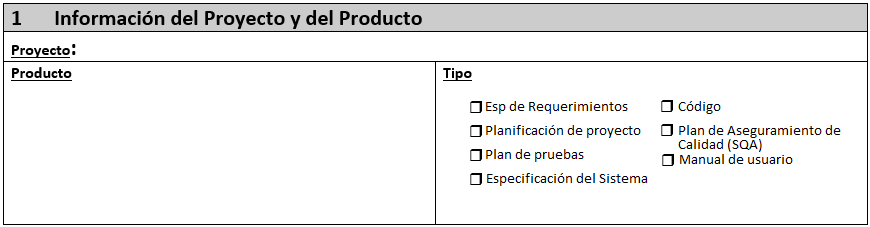
\includegraphics[width=1\textwidth]{figures/anexos/1-1.PNG}
\end{figure}

\begin{figure}[H]
\centering
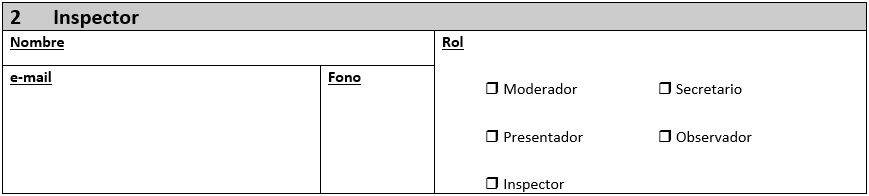
\includegraphics[width=1\textwidth]{figures/anexos/1-2.PNG}
\end{figure}

\begin{figure}[H]
\centering
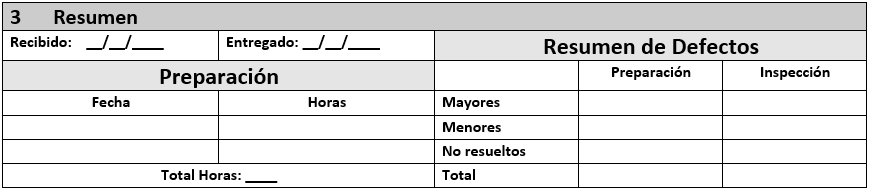
\includegraphics[width=1\textwidth]{figures/anexos/1-3.PNG}
\end{figure}

\begin{figure}[H]
\centering
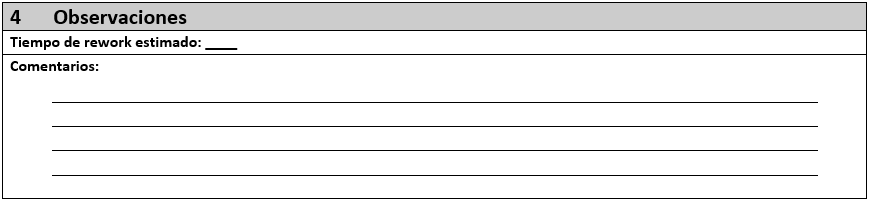
\includegraphics[width=1\textwidth]{figures/anexos/1-4.PNG}
\end{figure}

\begin{figure}[H]
\centering
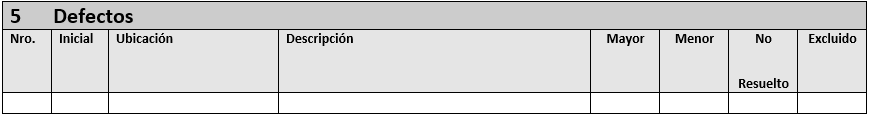
\includegraphics[width=1\textwidth]{figures/anexos/1-5.PNG}
\end{figure}

\section{Informe de Auditoria}

\begin{figure}[H]
\centering
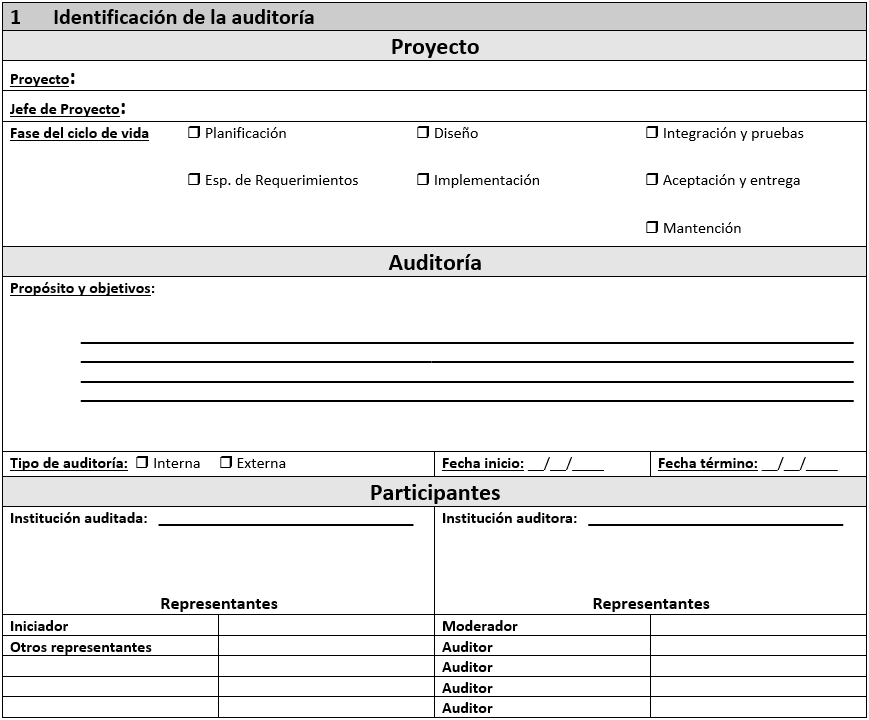
\includegraphics[width=1\textwidth]{figures/anexos/2-1.PNG}
\end{figure}

\begin{figure}[H]
\centering
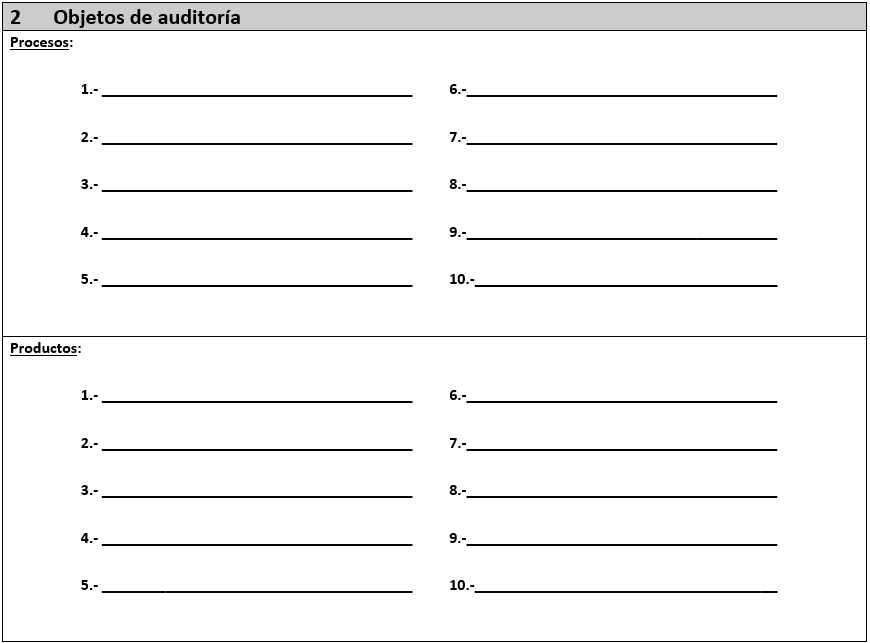
\includegraphics[width=1\textwidth]{figures/anexos/2-2.PNG}
\end{figure}

\begin{figure}[H]
\centering
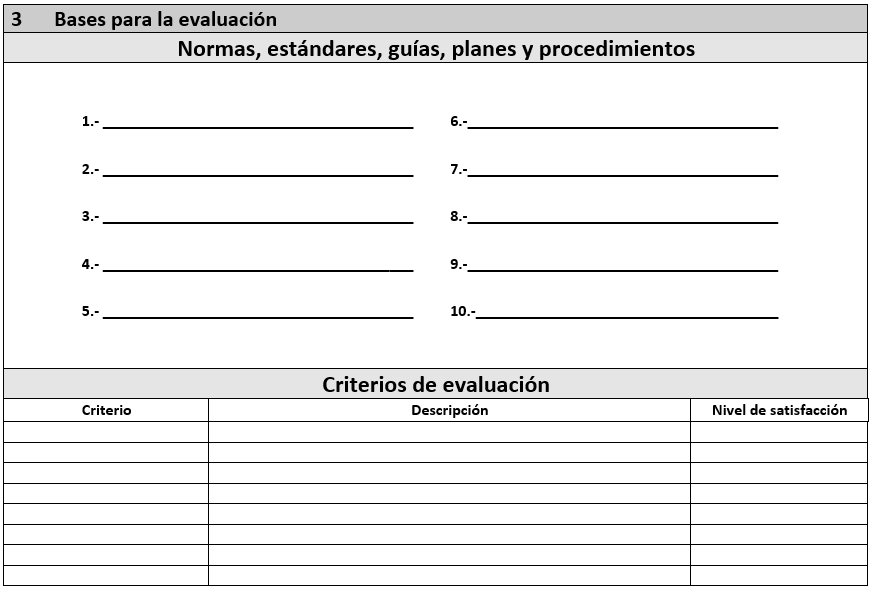
\includegraphics[width=1\textwidth]{figures/anexos/2-3.PNG}
\end{figure}

\begin{figure}[H]
\centering
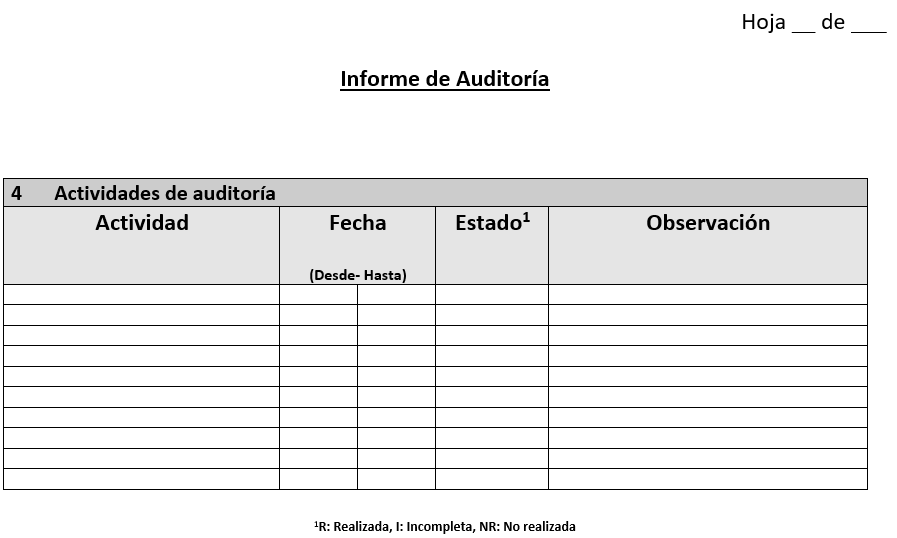
\includegraphics[width=1\textwidth]{figures/anexos/2-4.PNG}
\end{figure}

\begin{figure}[H]
\centering
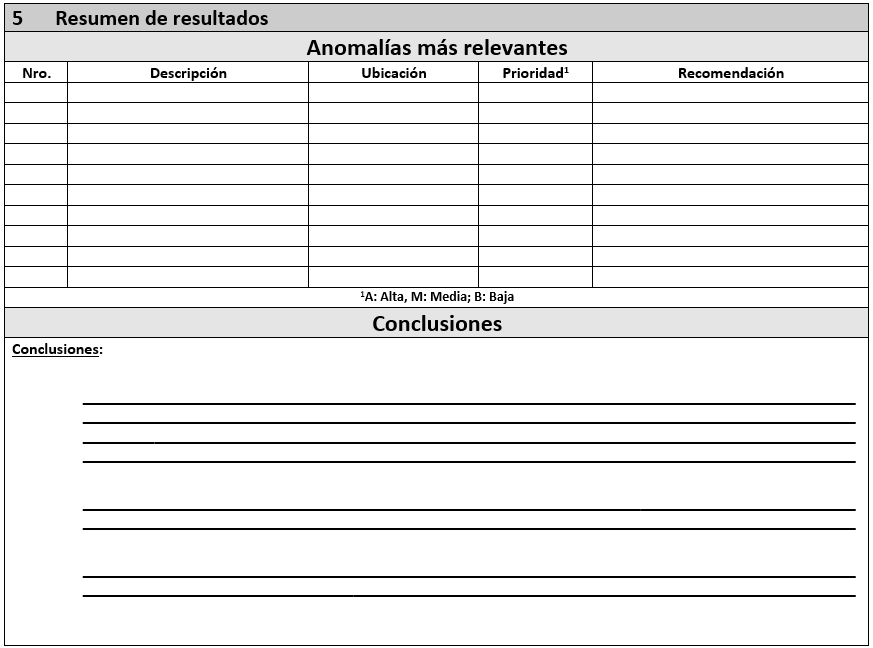
\includegraphics[width=1\textwidth]{figures/anexos/2-5a.PNG}
\end{figure}

\begin{figure}[H]
\centering
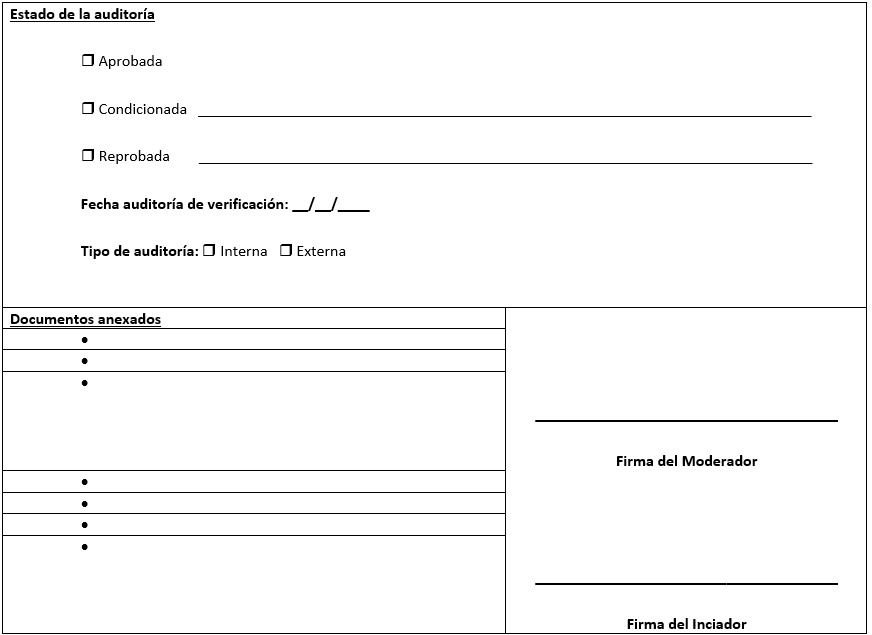
\includegraphics[width=1\textwidth]{figures/anexos/2-5b.PNG}
\end{figure}

\begin{figure}[H]
\centering
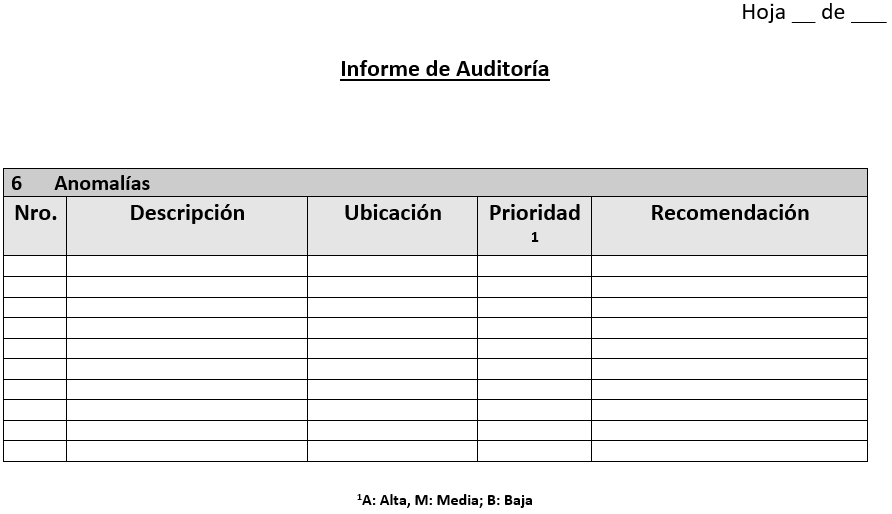
\includegraphics[width=1\textwidth]{figures/anexos/2-6.PNG}
\end{figure}

\section{Checklist}

\subsection{Checklist por actividades del proceso de desarrollo evaluados por QA}

\begin{figure}[H]
\centering
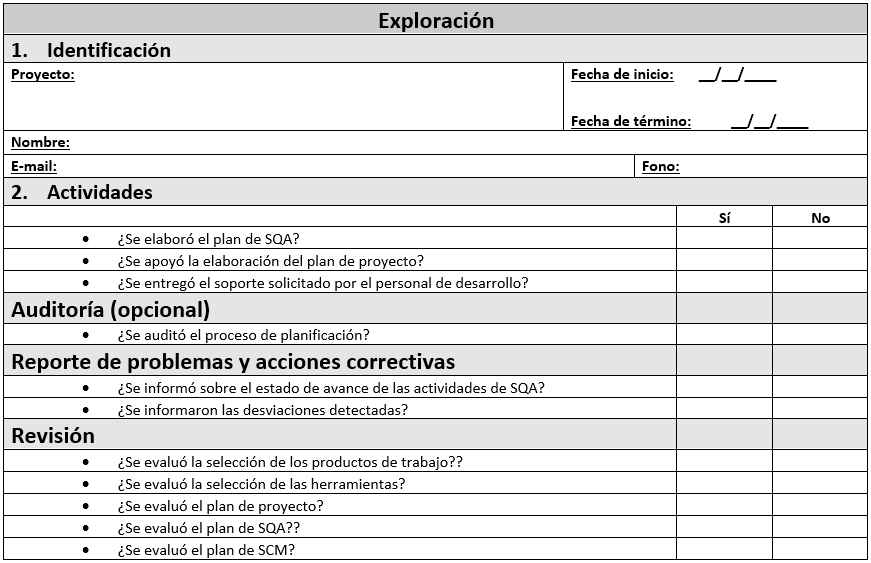
\includegraphics[width=1\textwidth]{figures/anexos/3-1-1.PNG}
\end{figure}

\begin{figure}[H]
\centering
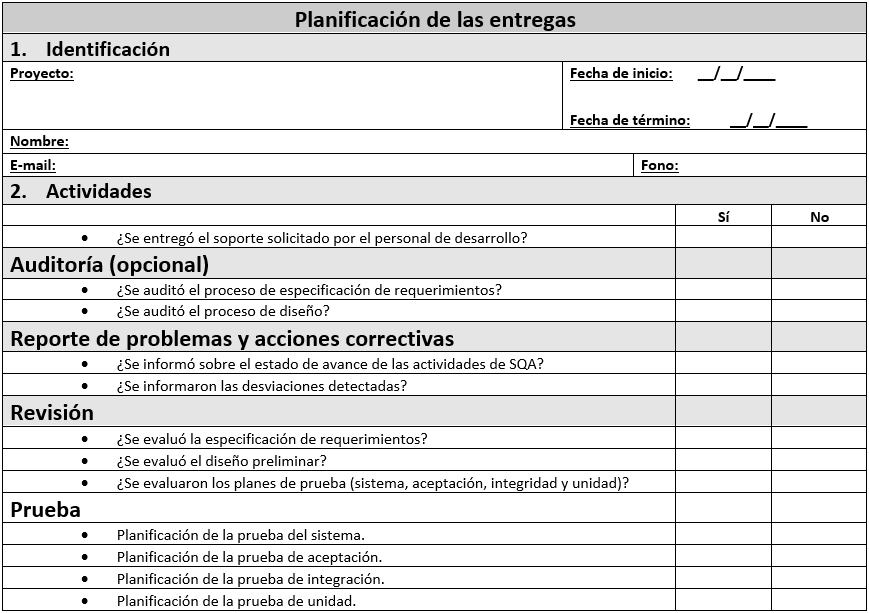
\includegraphics[width=1\textwidth]{figures/anexos/3-1-2.PNG}
\end{figure}

\begin{figure}[H]
\centering
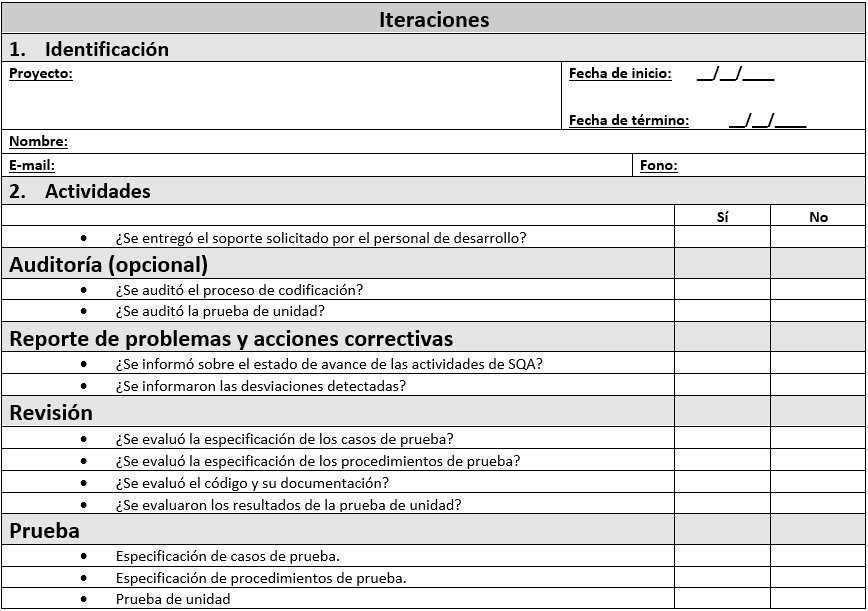
\includegraphics[width=1\textwidth]{figures/anexos/3-1-3.PNG}
\end{figure}

\begin{figure}[H]
\centering
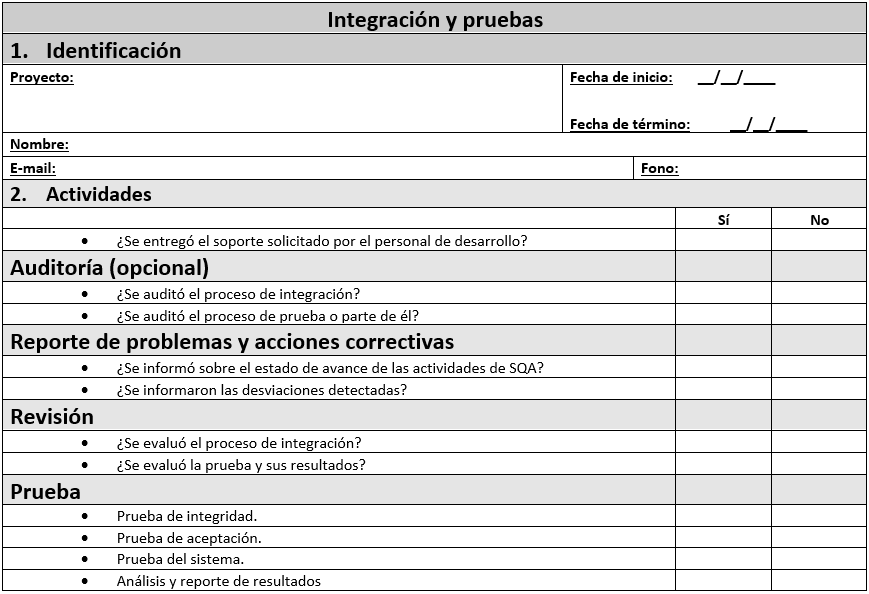
\includegraphics[width=1\textwidth]{figures/anexos/3-1-4.PNG}
\end{figure}

\begin{figure}[H]
\centering
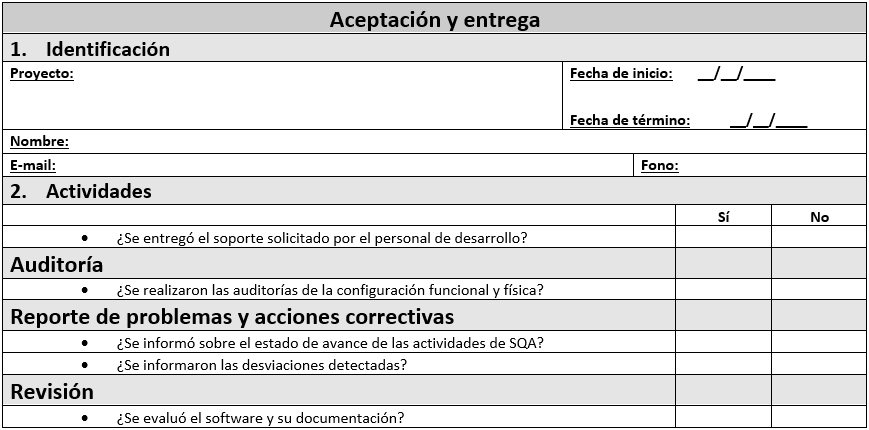
\includegraphics[width=1\textwidth]{figures/anexos/3-1-5.PNG}
\end{figure}

\begin{figure}[H]
\centering
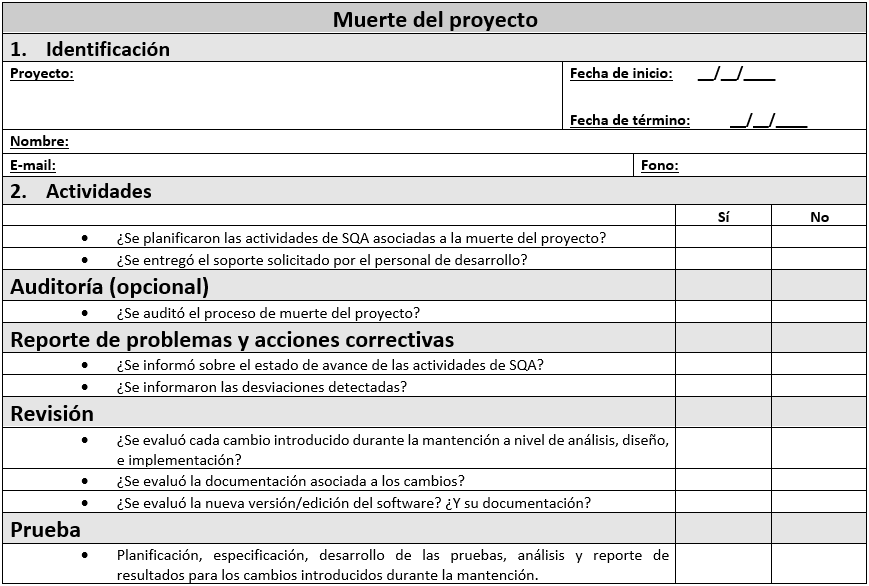
\includegraphics[width=1\textwidth]{figures/anexos/3-1-6.PNG}
\end{figure}

\subsection{Checklist por actividades del proceso de desarrollo evaluados por QA}

\begin{figure}[H]
\centering
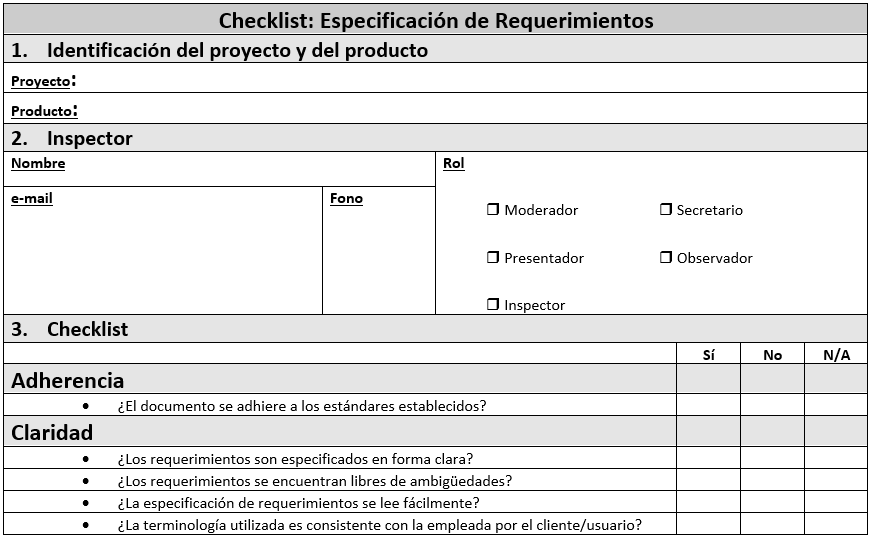
\includegraphics[width=1\textwidth]{figures/anexos/3-2-1a.PNG}
\end{figure}

\begin{figure}[H]
\centering
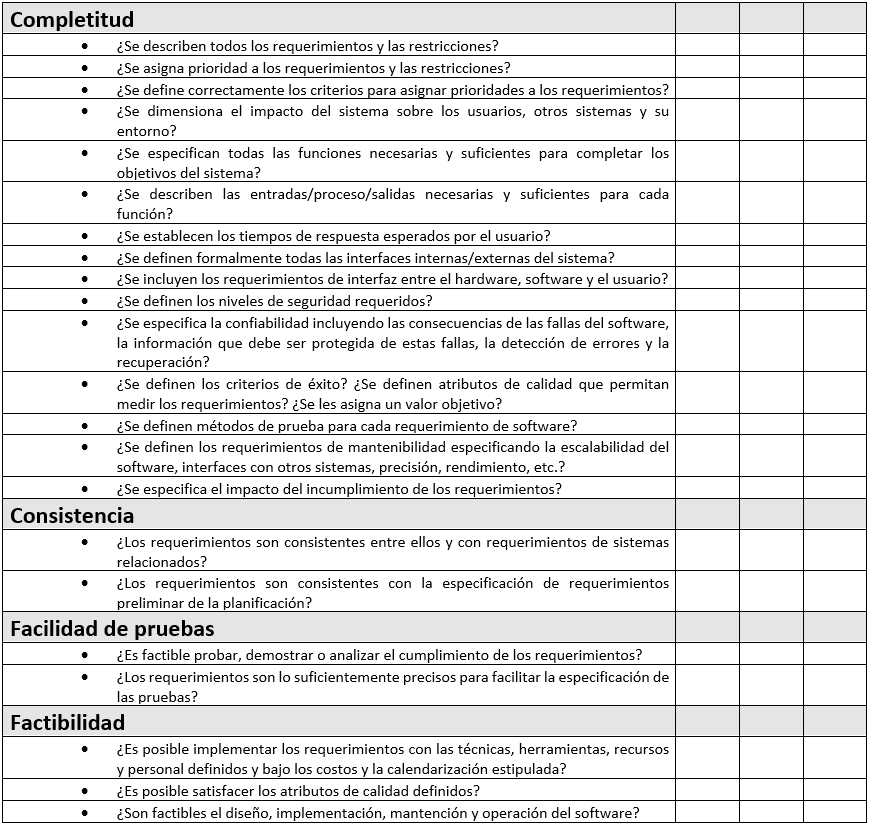
\includegraphics[width=1\textwidth]{figures/anexos/3-2-1b.PNG}
\end{figure}

\begin{figure}[H]
\centering
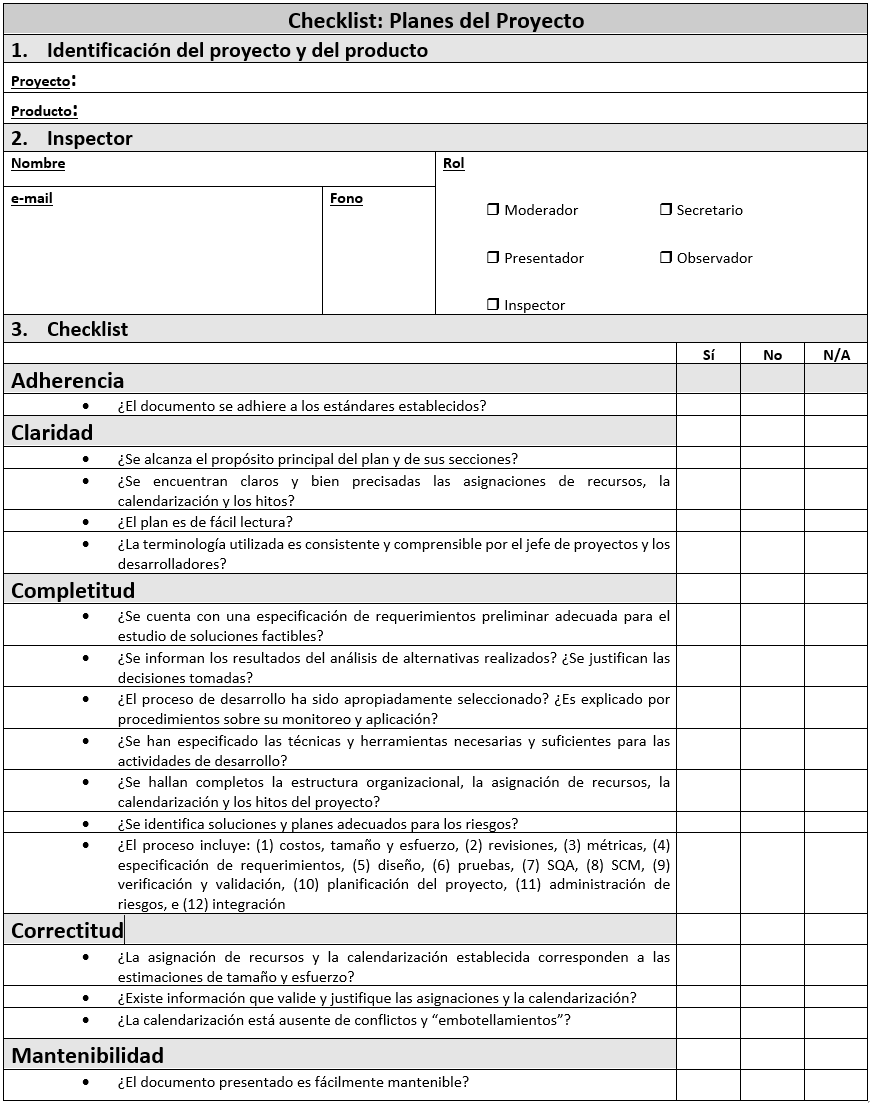
\includegraphics[width=1\textwidth]{figures/anexos/3-2-2.PNG}
\end{figure}

\begin{figure}[H]
\centering
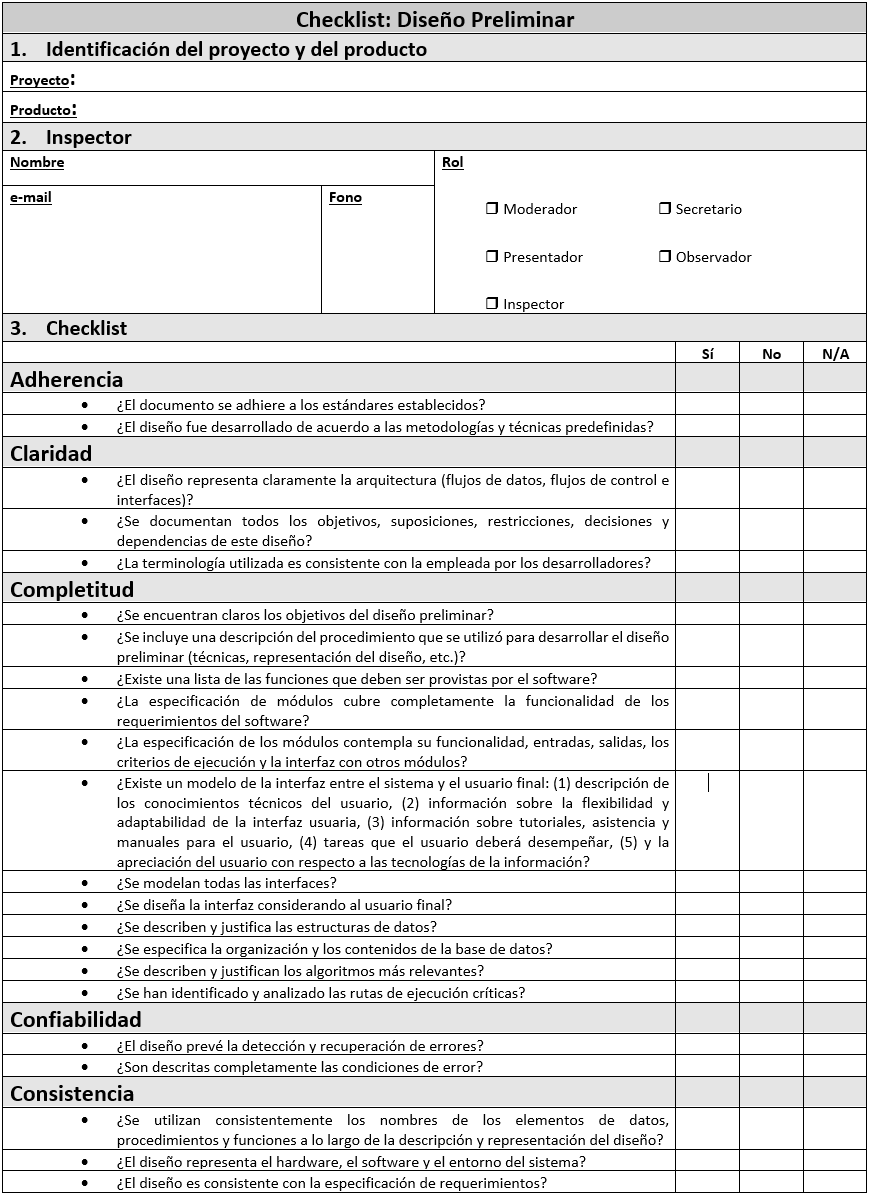
\includegraphics[width=1\textwidth]{figures/anexos/3-2-3a.PNG}
\end{figure}

\begin{figure}[H]
\centering
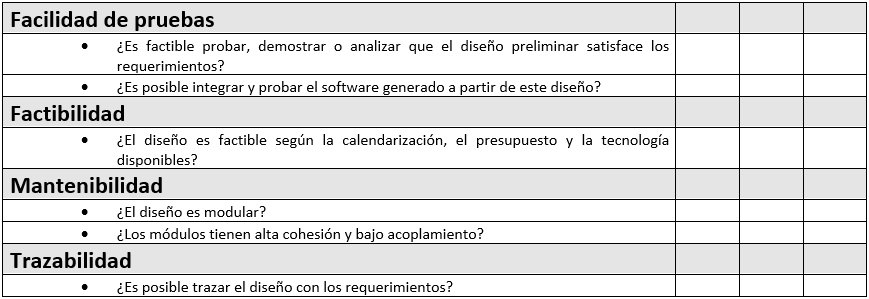
\includegraphics[width=1\textwidth]{figures/anexos/3-2-3b.PNG}
\end{figure}

\begin{figure}[H]
\centering
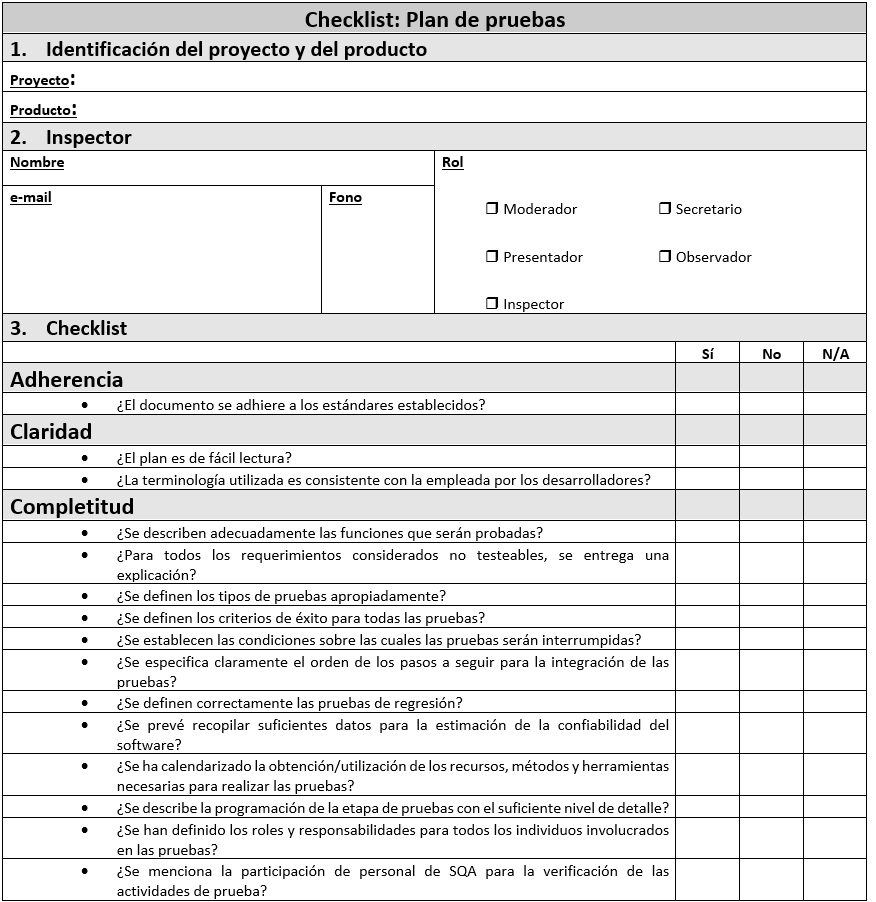
\includegraphics[width=1\textwidth]{figures/anexos/3-2-4a.PNG}
\end{figure}

\begin{figure}[H]
\centering
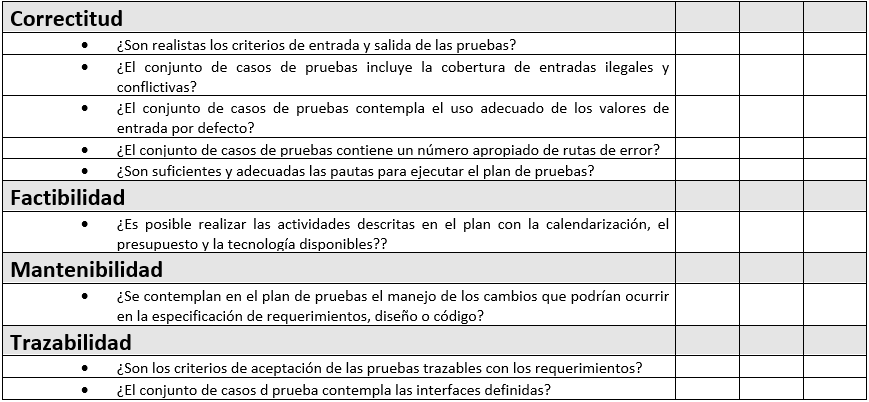
\includegraphics[width=1\textwidth]{figures/anexos/3-2-4b.PNG}
\end{figure}

\begin{figure}[H]
\centering
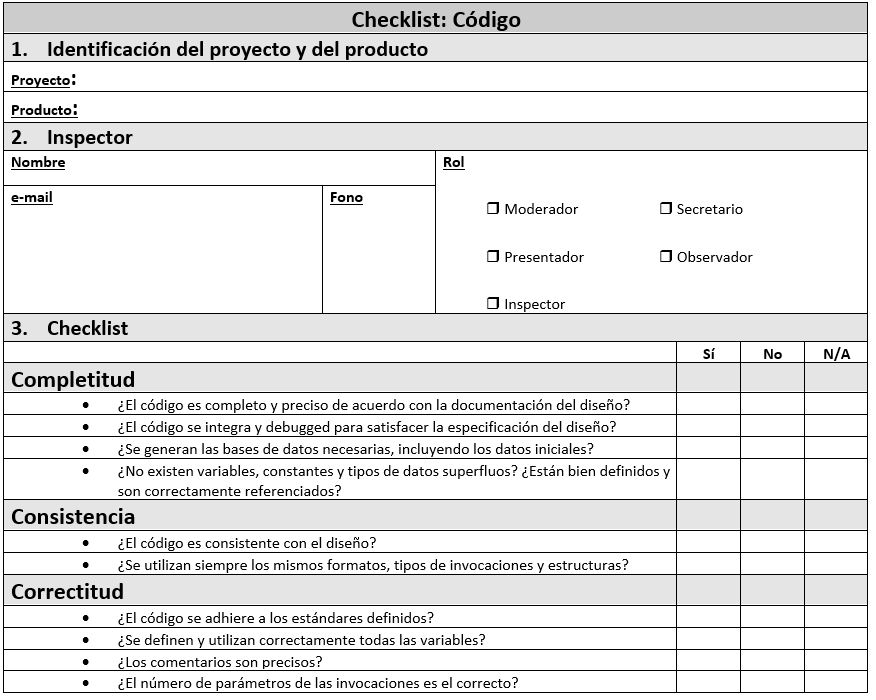
\includegraphics[width=1\textwidth]{figures/anexos/3-2-5a.PNG}
\end{figure}

\begin{figure}[H]
\centering
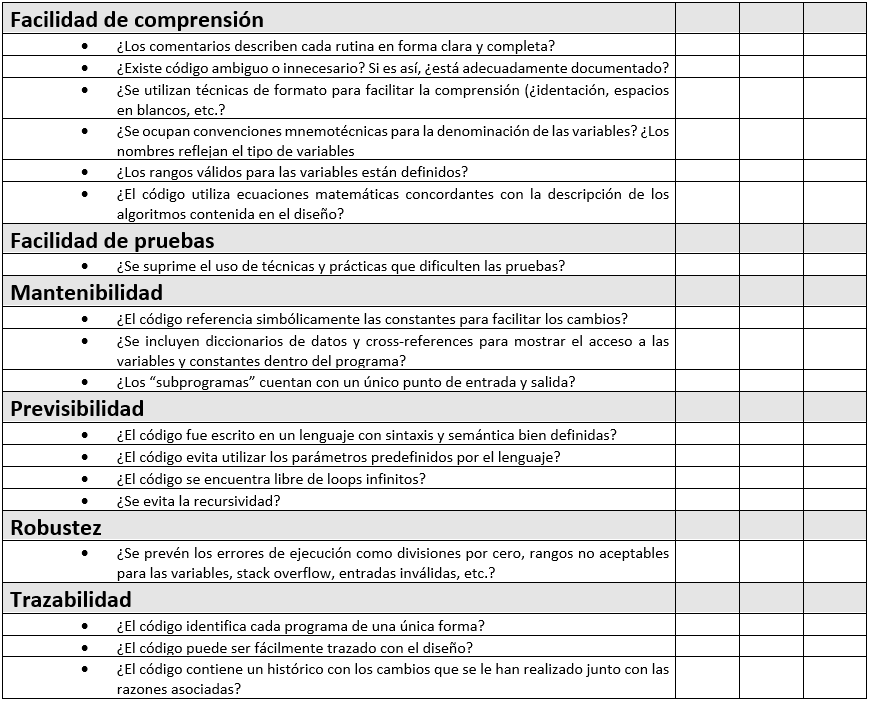
\includegraphics[width=1\textwidth]{figures/anexos/3-2-5b.PNG}
\end{figure}

\begin{figure}[H]
\centering
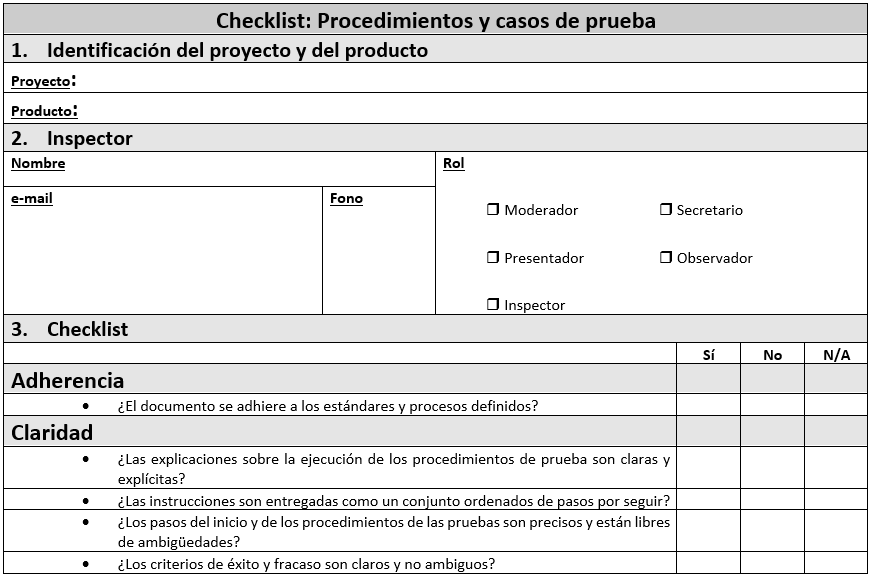
\includegraphics[width=1\textwidth]{figures/anexos/3-2-6a.PNG}
\end{figure}

\begin{figure}[H]
\centering
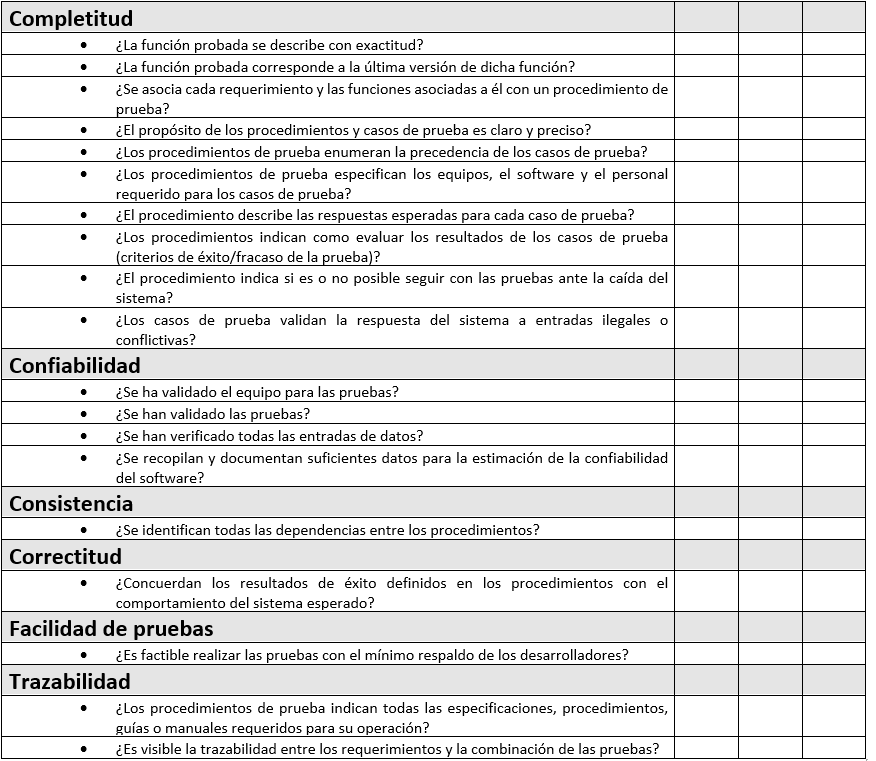
\includegraphics[width=1\textwidth]{figures/anexos/3-2-6b.PNG}
\end{figure}

\begin{figure}[H]
\centering
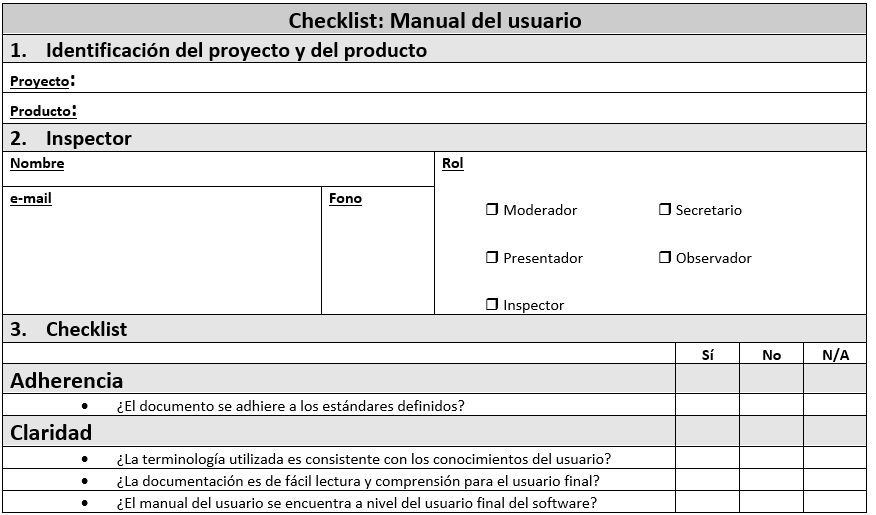
\includegraphics[width=1\textwidth]{figures/anexos/3-2-7a.PNG}
\end{figure}

\begin{figure}[H]
\centering
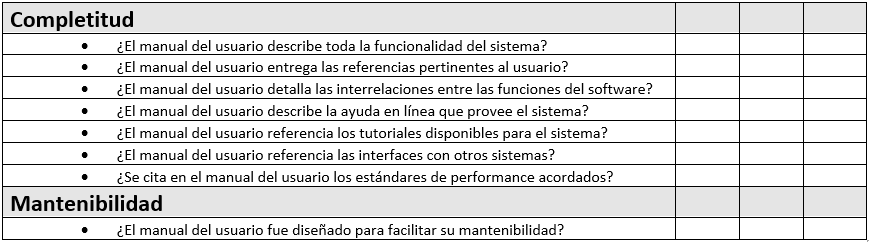
\includegraphics[width=1\textwidth]{figures/anexos/3-2-7b.PNG}
\end{figure}

\section{Checklist del Equipo de Revisión}

\begin{figure}[H]
\centering
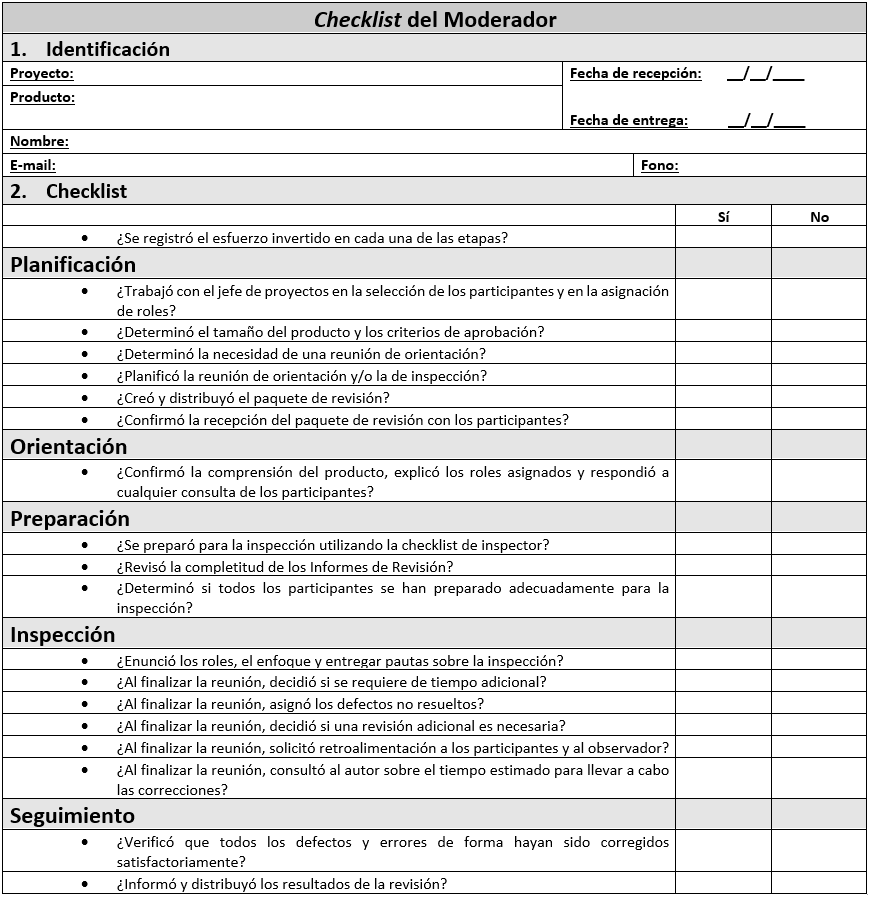
\includegraphics[width=1\textwidth]{figures/anexos/4-1.PNG}
\end{figure}

\begin{figure}[H]
\centering
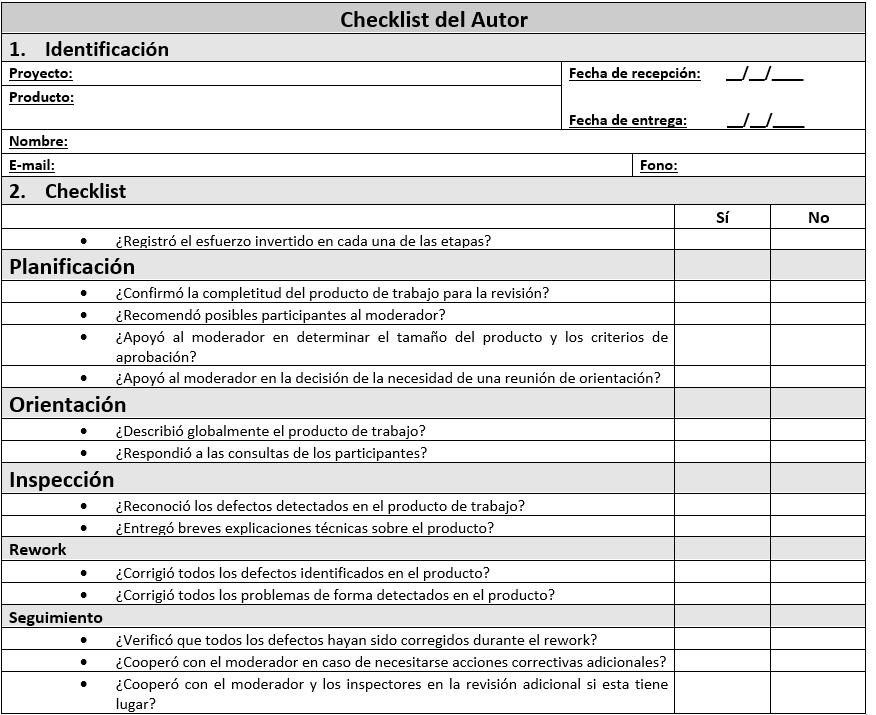
\includegraphics[width=1\textwidth]{figures/anexos/4-2.PNG}
\end{figure}

\begin{figure}[H]
\centering
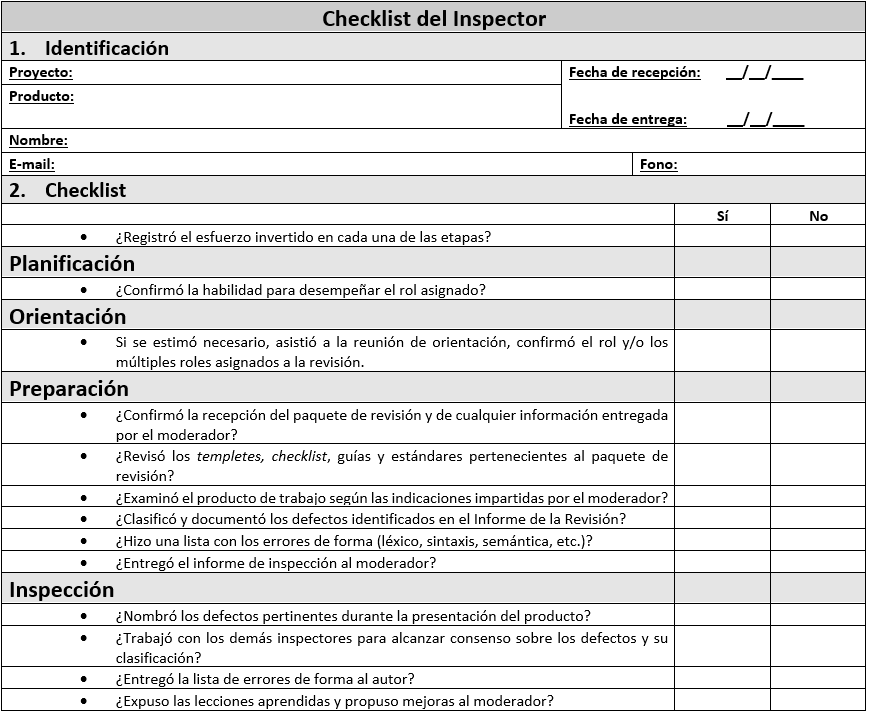
\includegraphics[width=1\textwidth]{figures/anexos/4-3.PNG}
\end{figure}

\begin{figure}[H]
\centering
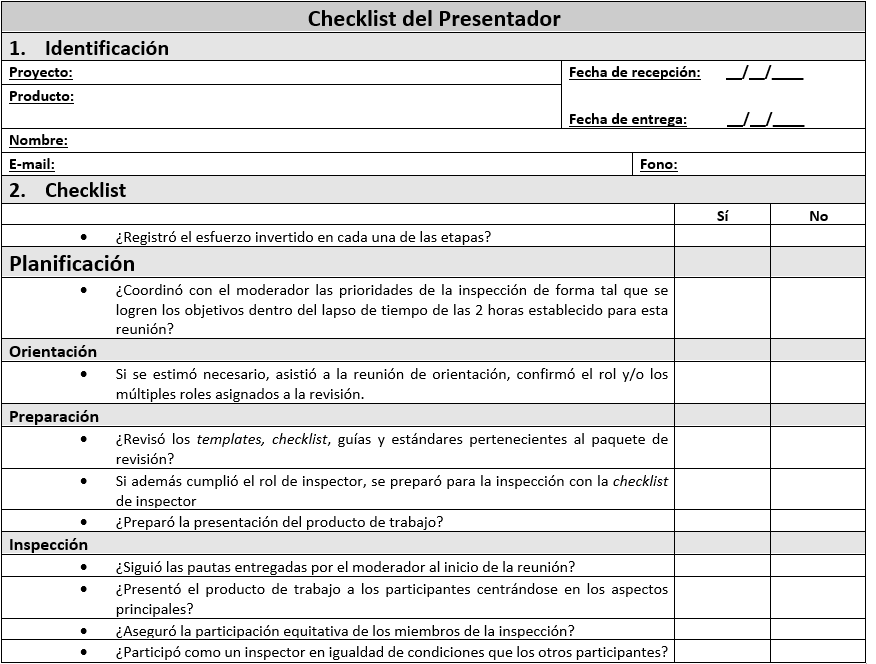
\includegraphics[width=1\textwidth]{figures/anexos/4-4.PNG}
\end{figure}

\begin{figure}[H]
\centering
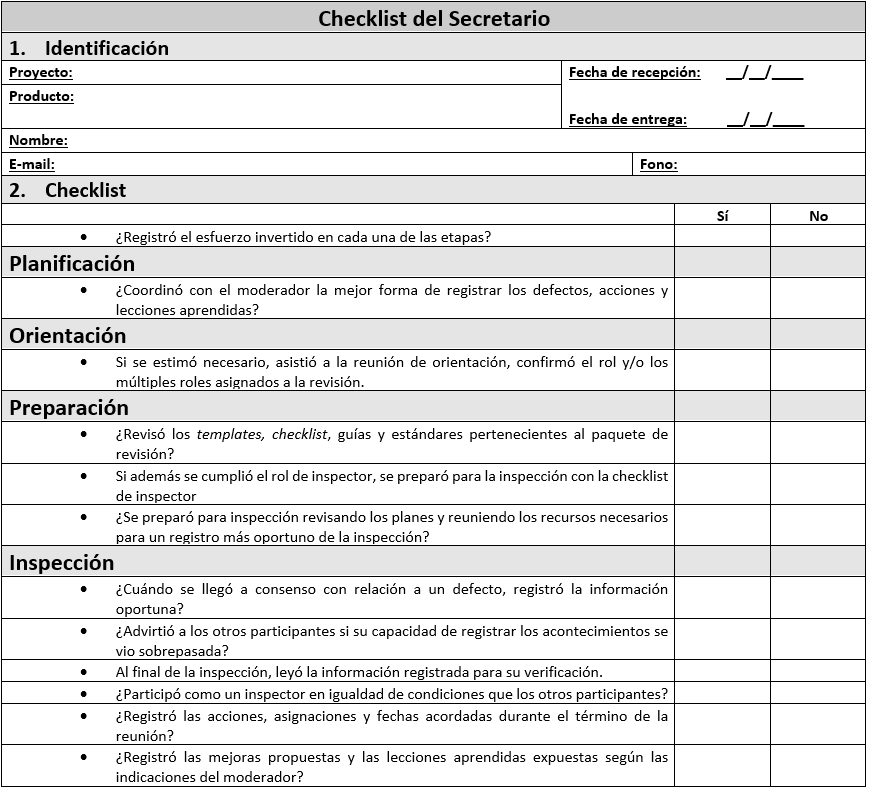
\includegraphics[width=1\textwidth]{figures/anexos/4-5.PNG}
\end{figure}

\begin{figure}[H]
\centering
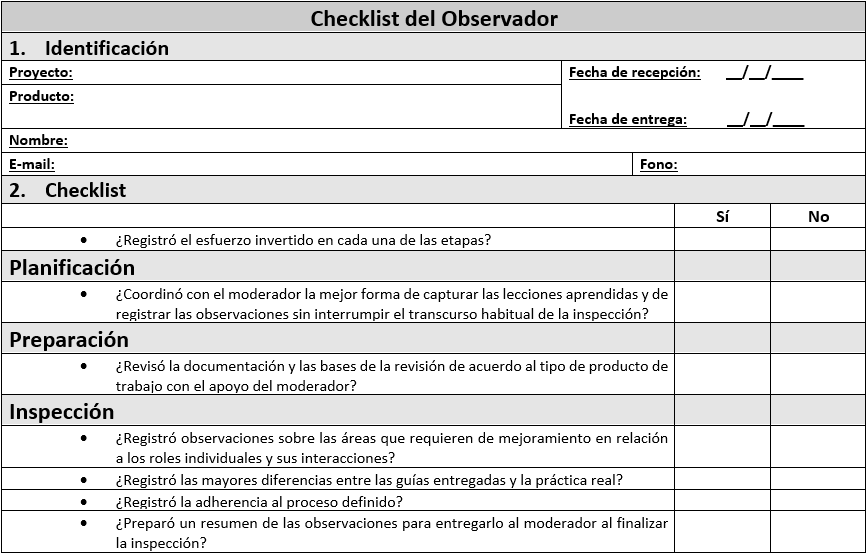
\includegraphics[width=1\textwidth]{figures/anexos/4-6.PNG}
\end{figure}

\section{Checklist del Equipo de Auditoria}

\begin{figure}[H]
\centering
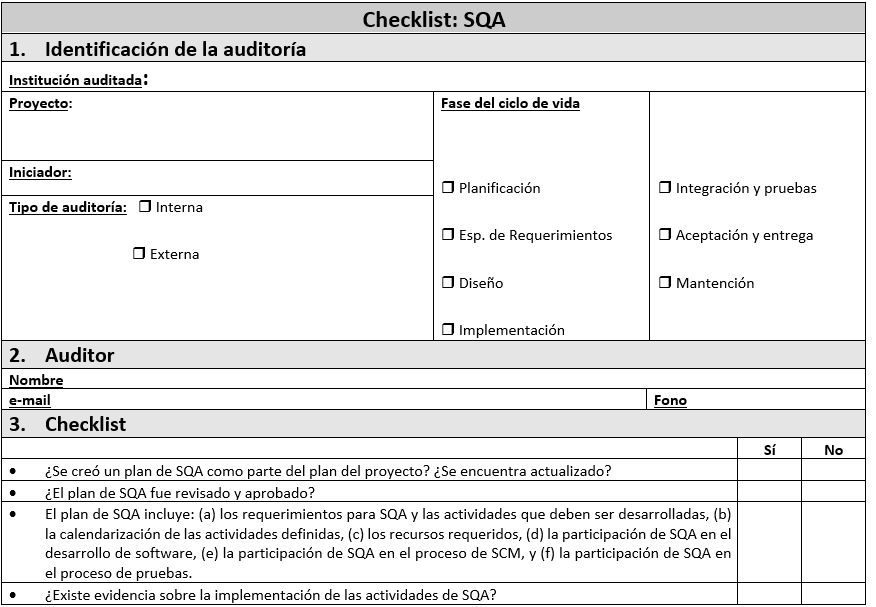
\includegraphics[width=1\textwidth]{figures/anexos/5-1.PNG}
\end{figure}

\begin{figure}[H]
\centering
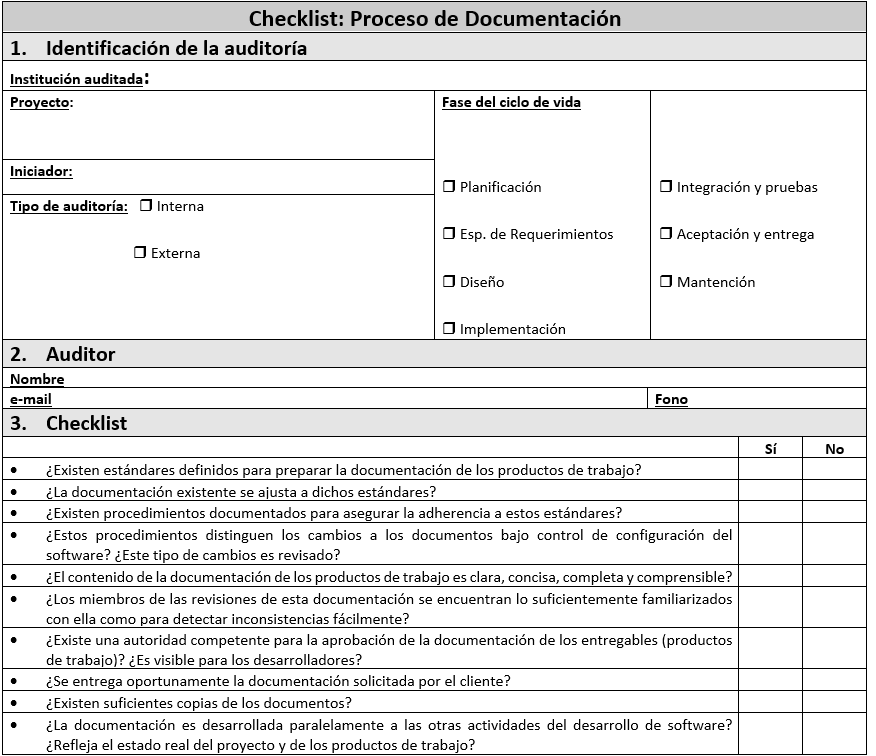
\includegraphics[width=1\textwidth]{figures/anexos/5-2.PNG}
\end{figure}

\begin{figure}[H]
\centering
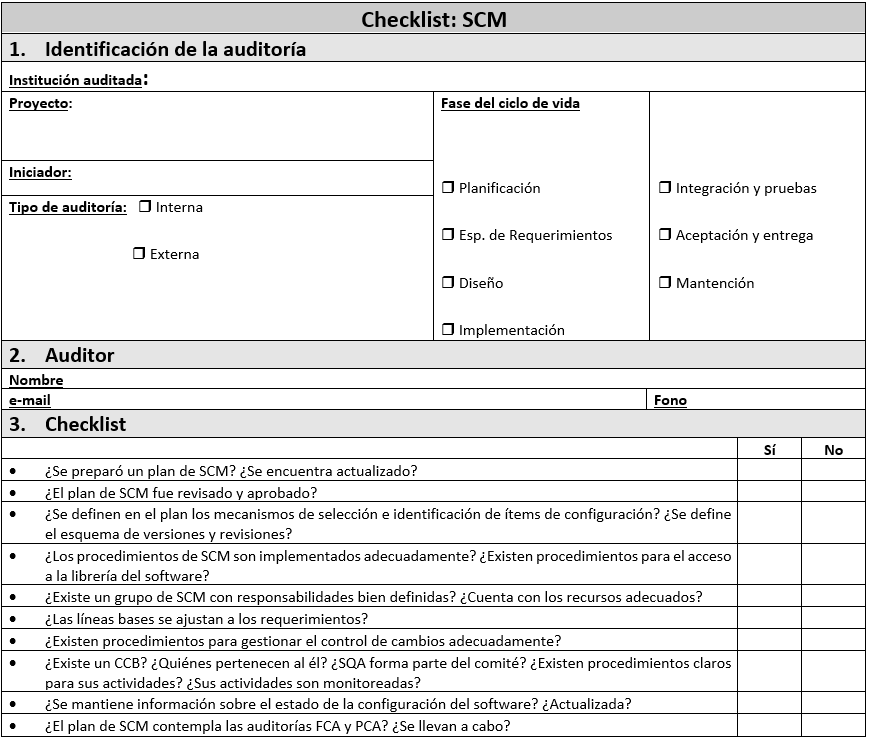
\includegraphics[width=1\textwidth]{figures/anexos/5-3.PNG}
\end{figure}

\begin{figure}[H]
\centering
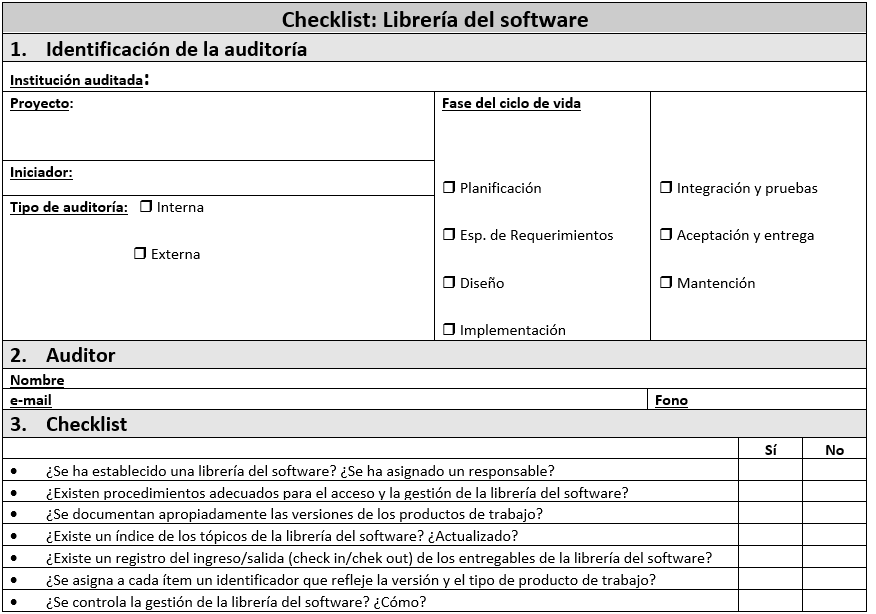
\includegraphics[width=1\textwidth]{figures/anexos/5-4.PNG}
\end{figure}

\begin{figure}[H]
\centering
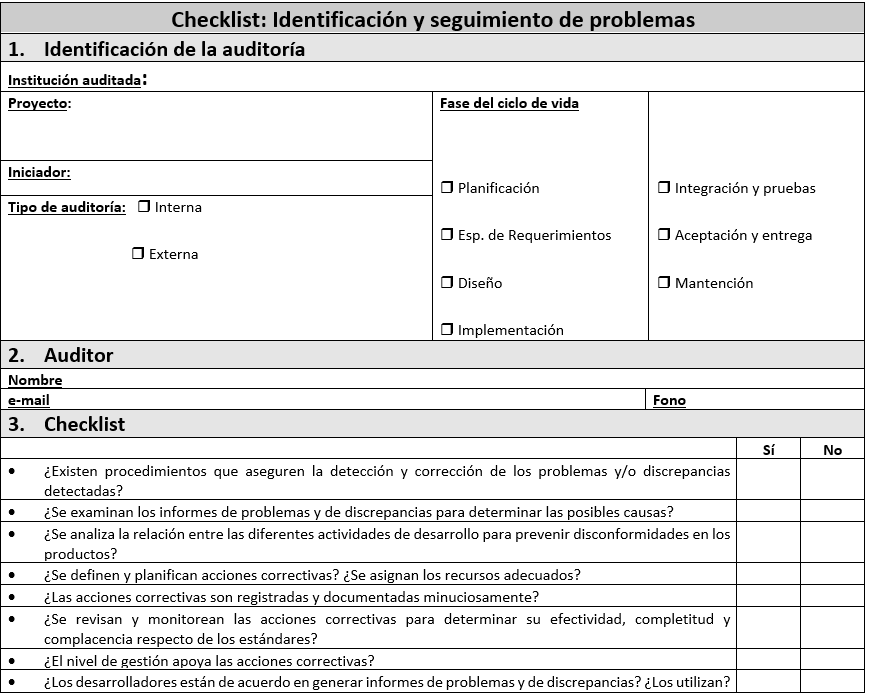
\includegraphics[width=1\textwidth]{figures/anexos/5-5.PNG}
\end{figure}

\begin{figure}[H]
\centering
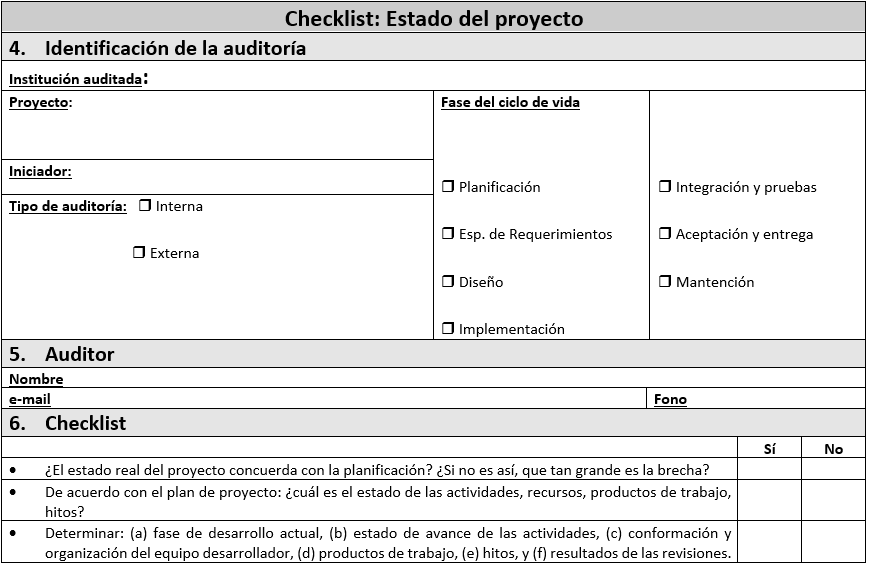
\includegraphics[width=1\textwidth]{figures/anexos/5-6.PNG}
\end{figure}

\section{Plantillas de pruebas}

\begin{figure}[H]
\centering
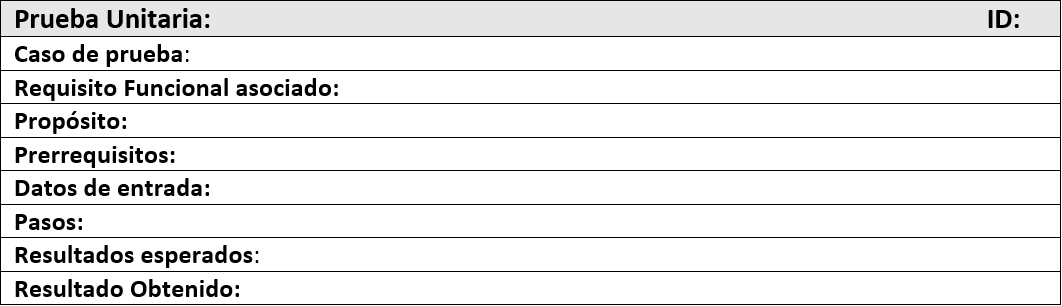
\includegraphics[width=1\textwidth]{figures/anexos/6-2-1-2.PNG}
\end{figure}

\begin{figure}[H]
\centering
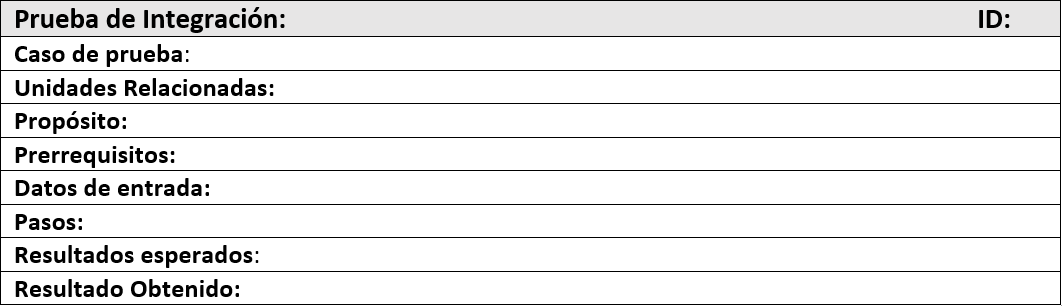
\includegraphics[width=1\textwidth]{figures/anexos/6-2-2-2.PNG}
\end{figure}

\begin{figure}[H]
\centering
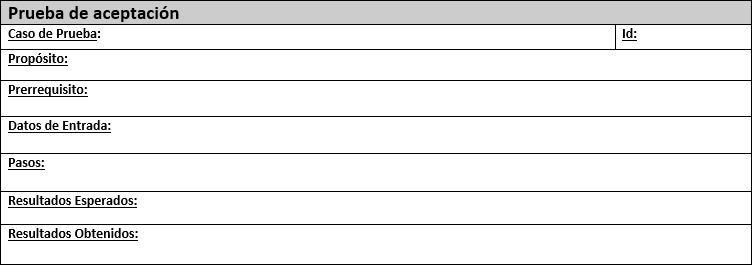
\includegraphics[width=1\textwidth]{figures/anexos/6-2-3-1.PNG}
\end{figure}

\begin{figure}[H]
\centering
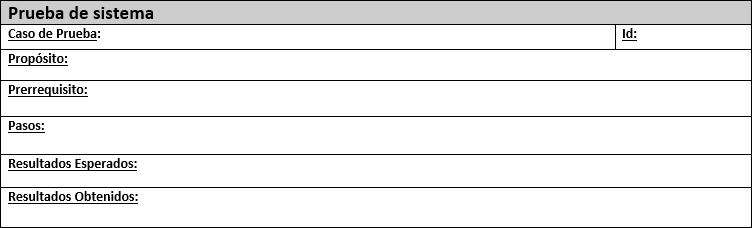
\includegraphics[width=1\textwidth]{figures/anexos/6-2-4-1.PNG}
\end{figure}
%...                  % Agregar más apéndices


\end{document}